\chapter{\texorpdfstring{Search for MSSM \AHtotautau}{Search for MSSM A/H -->tautau}}
\label{chap:mssm}

In this chapter the search for neutral Higgs bosons \PHiggs or \PHiggsps
decaying to a pair of \Pgt leptons will be discussed. The results presented
here correspond to those from an analysis peformed on 12.9 fb$^{-1}$ collected
at $\sqrt{s}=13$ TeV during the first half of the 2016 p--p running period of the \ac{LHC}, 
detailed in reference \cite{CMS-PAS-HIG-16-037}. The \etau, \mutau, \tautau and \emu final
states of the di-\Pgt pair were studied. The results of this search are 
model--independent upper limits on $\sigma \times$ BR of \PHiggs or \PHiggsps 
production in the two decay modes (see THEORY) and decay into $\Pgt\Pgt$. In 
addition, the results are interpreted in MSSM benchmark scenarios and 2D likelihood
scans of the two production modes are performed. A very similar analysis
was performed on 2.3 fb$^{-1}$ of data collected at $\sqrt{s}=13$ TeV during the 2015 \ac{LHC} p--p running period. 
As it is so similar to the analysis performed on the 2016 dataset it
will not be described in detail here, more information can be found in reference \cite{CMS-PAS-HIG-16-006}.
The results of the 2015 analysis will be shown, in addition to a combination of the 2015 and 2016 datasets.

For the analysis described in this chapter, as well as the 2015 analysis not detailed
here, I was responsible for optimisation of object selection and categorisation,
as well as studies of background methods for the \mutau, \etau and \tautau channels,
evaluation of systematic uncertainties in all four channels, and for producing
the statistical results, including model--dependent interpretations.

\section{Datasets and MC samples}
\label{sec:mssm_datasets}
The dataset used for this analysis corresponds to an integrated 
luminosity of 12.9 fb$^{-1}$ collected at a centre--of--mass
energy of 13 TeV during the first half of
the 2016 p--p running period of the \ac{LHC}. Section
\ref{sec:mssm_combination} includes the combination of this
dataset with a dataset collected during the 2015 p--p running
period of the \ac{LHC}. This dataset corresponds to an integrated
luminosity of 2.3 fb$^{-1}$ collected at $\sqrt{s} = 13$ TeV.

Signal and background events were generated using
various \ac{MC} event generators. Signal samples
for the $\Pg\Pg \rightarrow \phi$ and $\Pg\Pg \rightarrow b\bar{b}\phi$
production processes of $\PHiggs/\PHiggsps$ were generated using \texttt{PYTHIA 8.1} \cite{pythia81}.
These samples were produced in a range of masses between 90 GeV and 3.2 TeV.
This range is slightly wider than the range in which MSSM Higgs sector
benchmark computations are available, 90 GeV -- 2 TeV, and 
improves on the mass range, up to 1 TeV, studied during Run 1 in the context of BSM Higgs searches.
SM Higgs signal samples are used for the interpretation of the analysis results in 
MSSM benchmark scenarios. These samples are generated using \texttt{Powheg} \cite{powheg1,powheg2,powheg3}.

\ttbar- and single-top background samples are generated using \texttt{Powheg},
with \texttt{MadGraph5\_aMC\@NLO} \cite{amcnlo} used for the generation of di--boson background
samples and part of the W+$\gamma$ background included in the \emu channel only.
\Wjets and \Zll backgrounds are generated with the \ac{MadGraph 5} \cite{madgraph}
matrix element generator. Both samples containing a mixture
of jet multiplicities (`inclusive' samples) and samples with 1,2,3 or 4 jets (`exclusive' samples)
are generated. These exclusive samples increase the available number of
background events with higher jet multiplicities.  Part of the W+$\gamma$ background
samples are also generated with this event generator.
%note LO samples used because to get same number of effective
%events would need to generate more NLO samples
The `inclusive' and `exclusive' samples are reweighted
before they are combined so as to preserve the correct
fractions of events with each jet multiplicity.

Parton showering and hadronisation are modelled using \texttt{PYTHIA 8} for all 
samples. Minimum--bias events generated with \texttt{PYTHIA 8} are
added to all \ac{MC} samples to model additional interactions.

%THIS SECTION SHOULD JUST GO INTO THE DETAILED EVENT SELECTION
%SECTION
%\section{Optimisation of object selection}
%\label{sec:mssm_baseline_opt}
%At the start of Run 2 of the \ac{LHC} an effort was first made to
%optimise the default, \textit{baseline} di-\Pgt pair selection. This provides
%a common starting point for all $\PHiggs \rightarrow \Pgt\Pgt$ analyses, on
%top of which additional selections can be made for specific analyses such
%as the MSSM \AHtotautau analysis presented in this chapter. 

%\subsection{Electrons and muons}
%\label{sec:mssm_baseline_opt_elemu}
%For the optimisation of the baseline selection of
%electrons and muons the main optimisable
%selection is the choice of isolation discriminator and
%of 

\section{Event selection and categorisation}
\label{sec:mssm_eventsel}
In this section an overview of the event selection,
and how it was optimised, is given. More detailed information
on how the used objects used are reconstructed, 
and a more in--depth description of the identification criteria, 
is given in chapter \ref{chap:objects}.

\subsection{Pair selection and vetos}
\label{sec:mssm_eventsel_pairs}
The basis of the event selection is the selection of \mutau, \etau,
\tautau and \emu pairs following the requirements described
in the following subsections. After applying trigger
requirements, identification criteria and kinematic cuts
more than one possible candidate pair can exist. In this
case the pair is chosen as follows:
\begin{itemize}
\setlength{\itemsep}{-\baselineskip}
\item Prefer the pair with most isolated candidate 1 (muon for \mutau and \emu channels,
electron for \etau channel, either of the $\Pgt_h$s in \tautau channel). For electrons
and muons this means the object with the smallest relative isolation value is preferred, for $\Pgt_h$s the
object with raw MVA isolation value nearest to 1.
\item If the isolation of candidate 1 is the same in both pairs, prefer the pair with highest candidate 1 \pT.
\item If the \pT of candidate 1 is the same in both pairs, prefer the pair with most isolated
candidate 2 (e for the \emu channel, the other $\Pgt_h$ for the \tautau channel, 
and the $\Pgt_h$ for \etau and \mutau channels).
\item If the isolation of candidate 2 is the same in both pairs, prefer the pair with highest candidate 2 \pT.
\end{itemize}

To prevent overlap with other channels, events are rejected
if there are muons and electrons, other than those in the selected pair,
with \pT $>10$ GeV and passing loose ID and isolation requirements.
This also reduces backgrounds from \WZ events. 
In addition to this, \Zee events are 
reduced in the \etau channel by rejecting events
where an opposite--sign pair of electrons of \pT $>15$ GeV
and passing very loose ID and isolation requirements can be formed. 
In the \mutau channel the contribution from \Zmm events
is reduced in a similar fashion. 




\subsection{\texorpdfstring{Event selection in the \mutau channel}{Event selection in the mu tau channel}}
\label{sec:mssm_eventsel_mt}
The first selection layer in the \mutau channel is a trigger
that only requires a muon at \ac{L1}. At the level of the \ac{HLT}, 
loose identification and isolation criteria are then applied to this muon.

The offline event selection proceeds to require an oppositely charged
muon and hadronically decaying tau, which are well--separated ($\Delta R > 0.5$).
The minimum \pT of the muon is required to be 23 GeV, with $|\eta| < 2.1$. %due to trigger conditions
Additional ``medium'' identification requirements are placed on the muon, in addition
to requiring the muon to be consistent with having originated from the primary vertex, such that
the impact parameters $d_{xy} < 0.045$ cm and $d_{z} < 0.2$ cm. The muon is also required
to be isolated, with a selection on its relative isolation variable calculated with a cone size of 0.4 of $< 0.15$.

The hadronic tau needs to have a \pT greater than 30 GeV, $|\eta|<2.3$,
is required to be reconstructed by the HPS algorithm and to pass the medium
working point of the MVA isolation discriminator. The hadronic tau also needs
to have originiated from the primary vertex and so the impact paramter $d_{z}$ is 
required to be less than 0.2 cm. Finally the hadronic tau is required
to satisfy the very loose working point of the anti--electron discriminator
and the tight working point of the anti--muon discriminator.

The selection on the muon's relative isolation is chosen after comparing
the performance of several isolation variables at different
relative isolation values. This was based on a simple \mutau channel
event selection as described above, with varying isolation variables.
The selection was optimised based on two figures of merit, both of
which consider \Ztautau as the signal and the other backgrounds
as background. The first figure of merit used is the number of signal events divided by the
square root of the number of background events, $S/\sqrt{B}$, after
the selection. The aim with this figure of merit is to choose
the isolation selection that maximises it. The second figure of merit
is the uncertainty interval on the best-fit value for a maximum--likelihood fit
to the \Ztautau signal strength, which should be minimised by the choice of
isolation selection.

Different isolation variables were studied over a range of values
to cut at. In addition to the $\Delta\beta$ corrected isolation variable analogous
to the one given for electrons in equation \ref{eqn:electron_reliso} with 
isolation cone sizes in $\Delta R$ of 0.3 and 0.4, a very similar
variable which does not just consider charged \ac{PF} hadrons, but
also electrons and muons in the isolation sum is considered. This
variable is also studied for both cone sizes of 0.3 and 0.4. Finally,
a relative isolation variable based solely on the \pT of tracks from the primary
vertex,
\begin{equation}\label{eqn:reltrkiso}
I_{\text{trk}} = \frac{\Sigma p_{\text{T}}^{\text{tracks from PV within cone of 0.3 of the muon}}}{p_{\text{T}}^{\mu}}, \end{equation} 
is studied. The $S/\sqrt{B}$ for the different isolation variables is shown in figure \ref{fig:mssm_selection_mt_muons}a, with the
size of the error interval from the maximum--likelihood fit to the \Ztautau signal strength shown in 
\ref{fig:mssm_selection_mt_muons}b. From the fact that both figures of merit do not
vary so much with different isolation cuts and different variables we can see that this analysis
is not so sensitive to fake,nonisolated muons. The choice of isolation variable is therefore
driven mostly by simplicity and consistency with other \ac{CMS} analyses.

\begin{figure}[h!]
\begin{center}
\subfloat[$S/\sqrt{B}$]{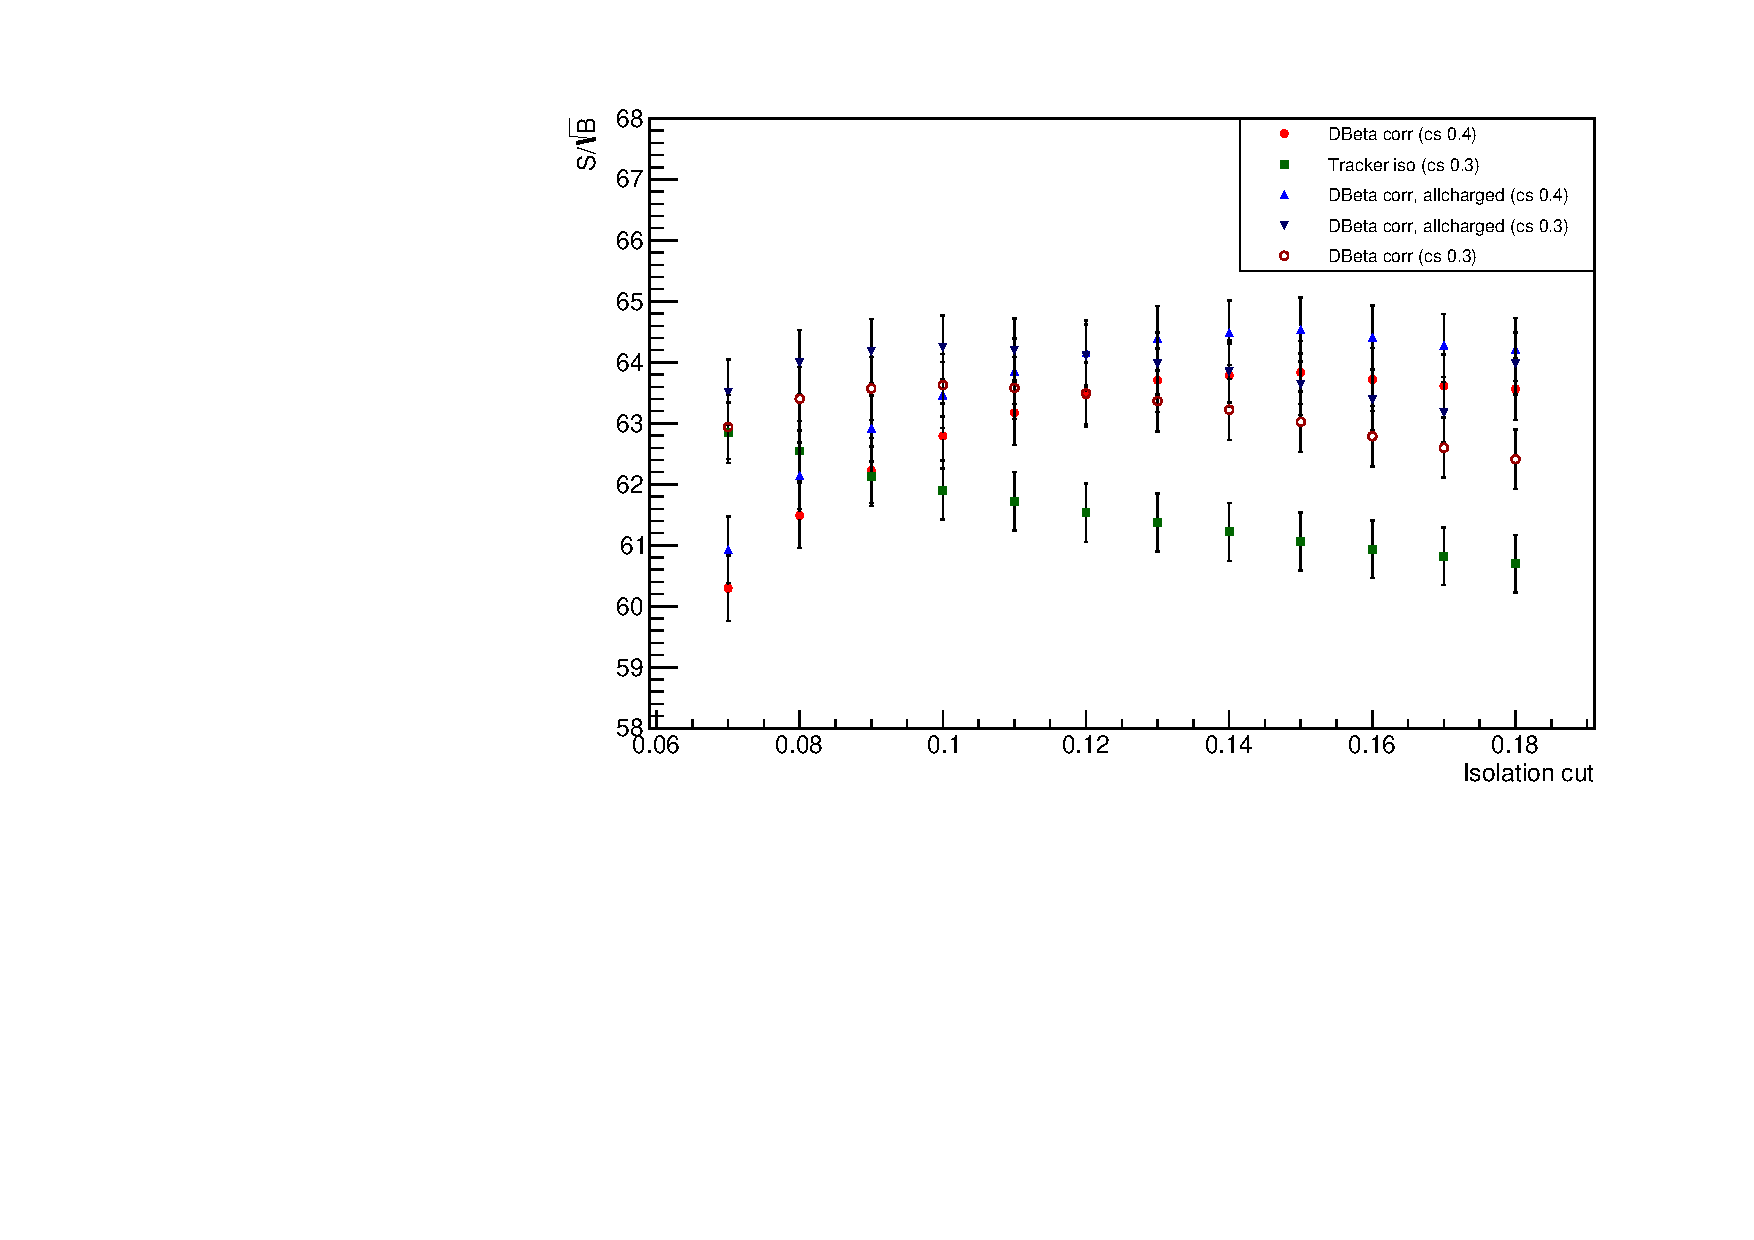
\includegraphics[width=0.7\textwidth]{./MSSM/Figures/s_over_root_b_mt_m.pdf}}~\\
\subfloat[Size of error interval]{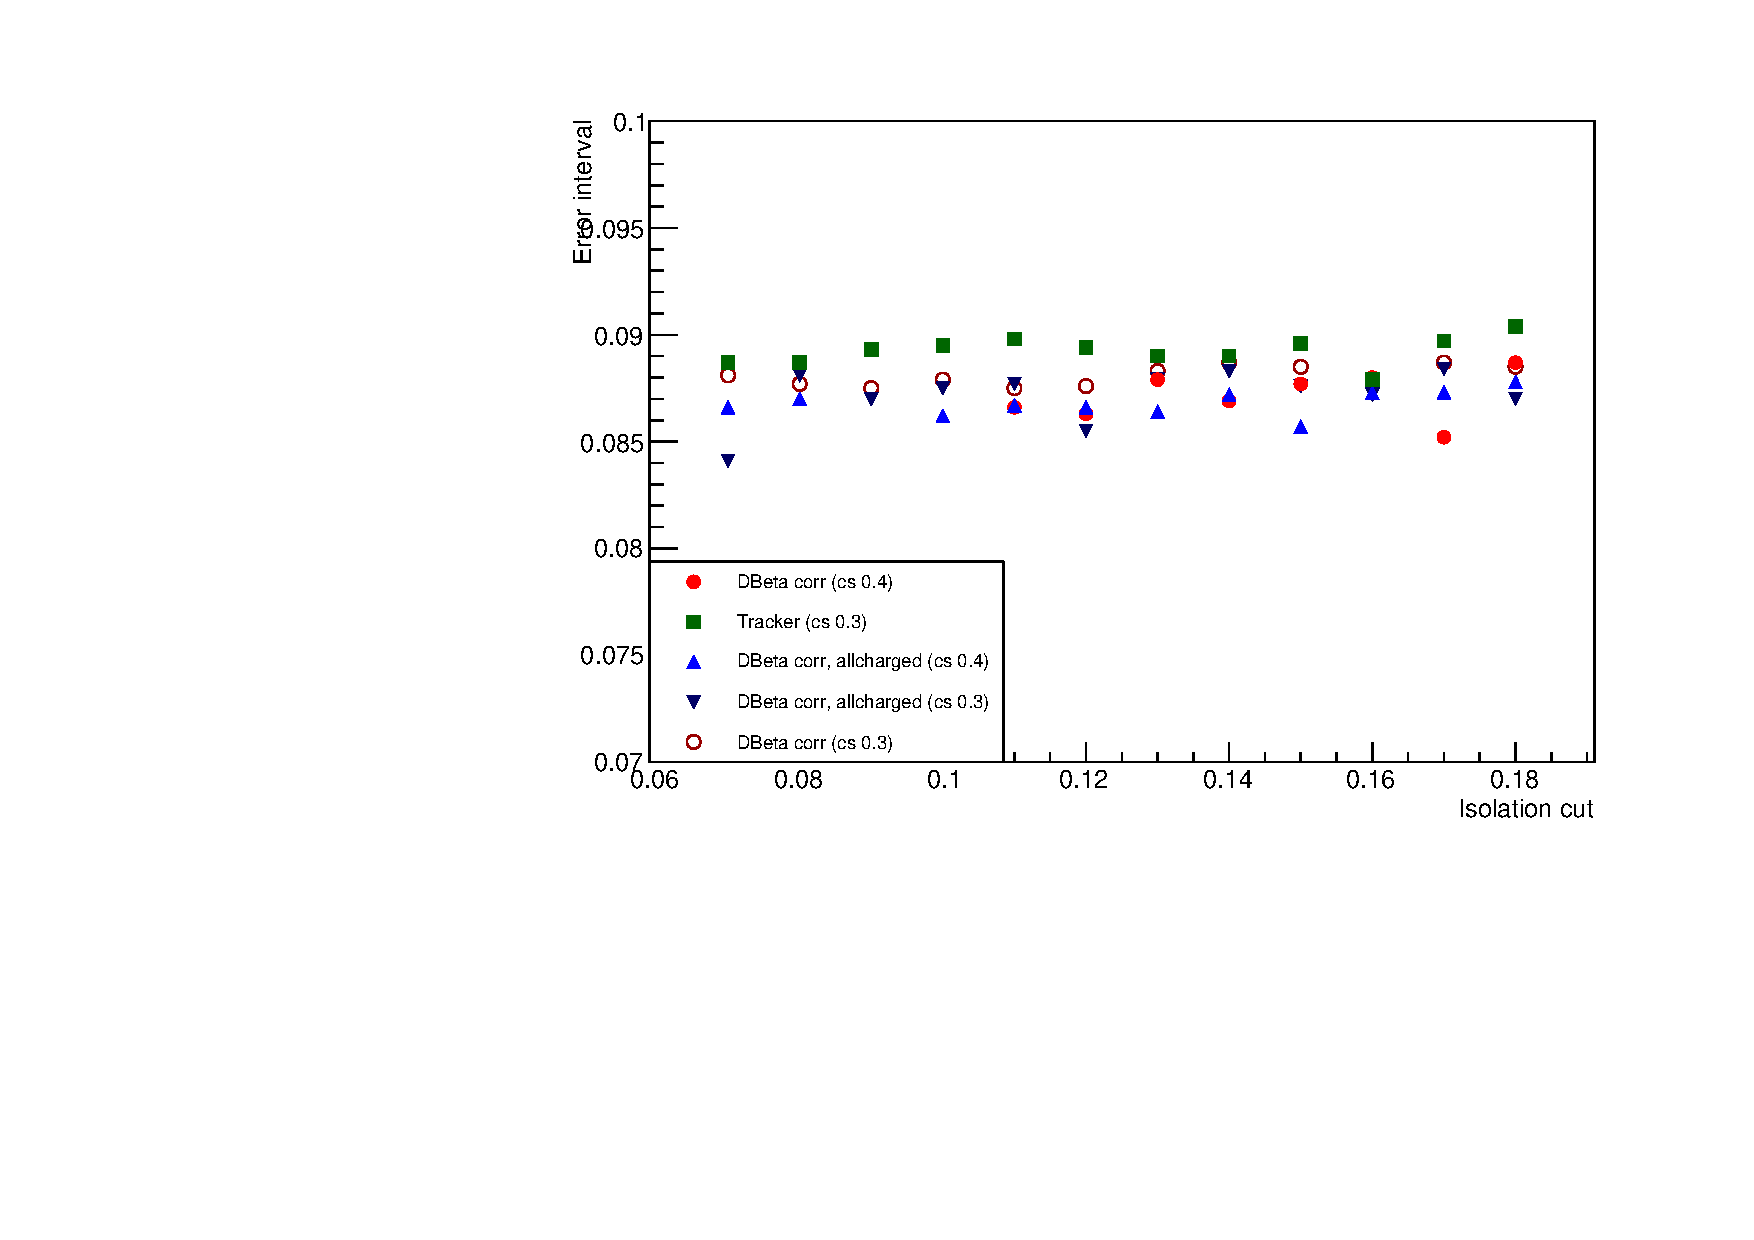
\includegraphics[width=0.7\textwidth]{./MSSM/Figures/mt_muons_iso_errint.pdf}}
\end{center}
\caption{(a) The $S/\sqrt{B}$ for \Ztautau signal and (b) the size of the error interval on 
the best--fit value of a maximum--likeihood fit to the \Ztautau signal strength,
for various cut values of the $\Delta\beta$--corrected
isolation variable with a cone size of $\Delta R = 0.4$ (solid circles), 
the $\Delta\beta$--corrected isolation variable with a cone size of $\Delta R = 0.3$ (open circles),
the $\Delta\beta$--corrected isolation variable including electrons and muons in the isolation
sum, for a cone size of $\Delta R =0.4$ (upward facing triangles) and $\Delta R =0.3$ (downward facing triangles) and
the tracker--based relative isolation (solid squares).}
\label{fig:mssm_selection_mt_muons}
\end{figure}

A topological selection on the \mT~variable, 
introduced in section \ref{sec:hhh_selection_categories}, is made on 
events in the \mutau channel. This selection and the
choice of hadronic tau isolation working point interfere 
with each other and therefore they are optimised in a 2D--optimisation. 
The pre--fit expected upper limits on $\sigma\times$BR for both gg$\phi$ and bb$\phi$
production with decay into $\Pgt\Pgt$ at several mass points 
in the 90 GeV -- 3.2 TeV range are used to do this. 
Because of the use of such a wide range of signal masses, it
is not possible to choose a selection that is optimal
for every mass point. This is illustrated in figure \ref{fig:mssm_selection_mt_taumt}:
figure \ref{fig:mssm_selection_mt_taumt}a shows the upper limit on $\sigma\times$BR for
the gluon--gluon fusion production process, at a mass $m_{\phi} = 160$ GeV, with
figures \ref{fig:mssm_selection_mt_taumt}b,c and d showing this upper limit at $m_{\phi} = 900$ GeV,
$m_{\phi} = 1600$ GeV and $m_{\phi} = 2900$ GeV respectively. From these figures
we can observe that looser selections are preferred for higher masses. This can be
explained by considering the function of each of the selections. Tightening the hadronic
tau isolation working point reduces the selection of fake taus and increases the proportion
of backgrounds which contain real hadronic taus. The \mT~selection reduces
the \Wjets background. As the backgrounds are concentrated at the lower
end of the spectrum of mass--like discriminating variables, such tighter
selections are preferred where signal and backgrounds overlap. However, at higher
mass points the signal--sensitive range of the discriminating variable is 
low in backgrounds and there is more benefit to loosening the selection
to increase the signal efficiency than to keep the tighter selection
to reduce an already low background.

\begin{figure}[h!]
\begin{center}
\subfloat[$m_{\phi} = 160$ GeV]{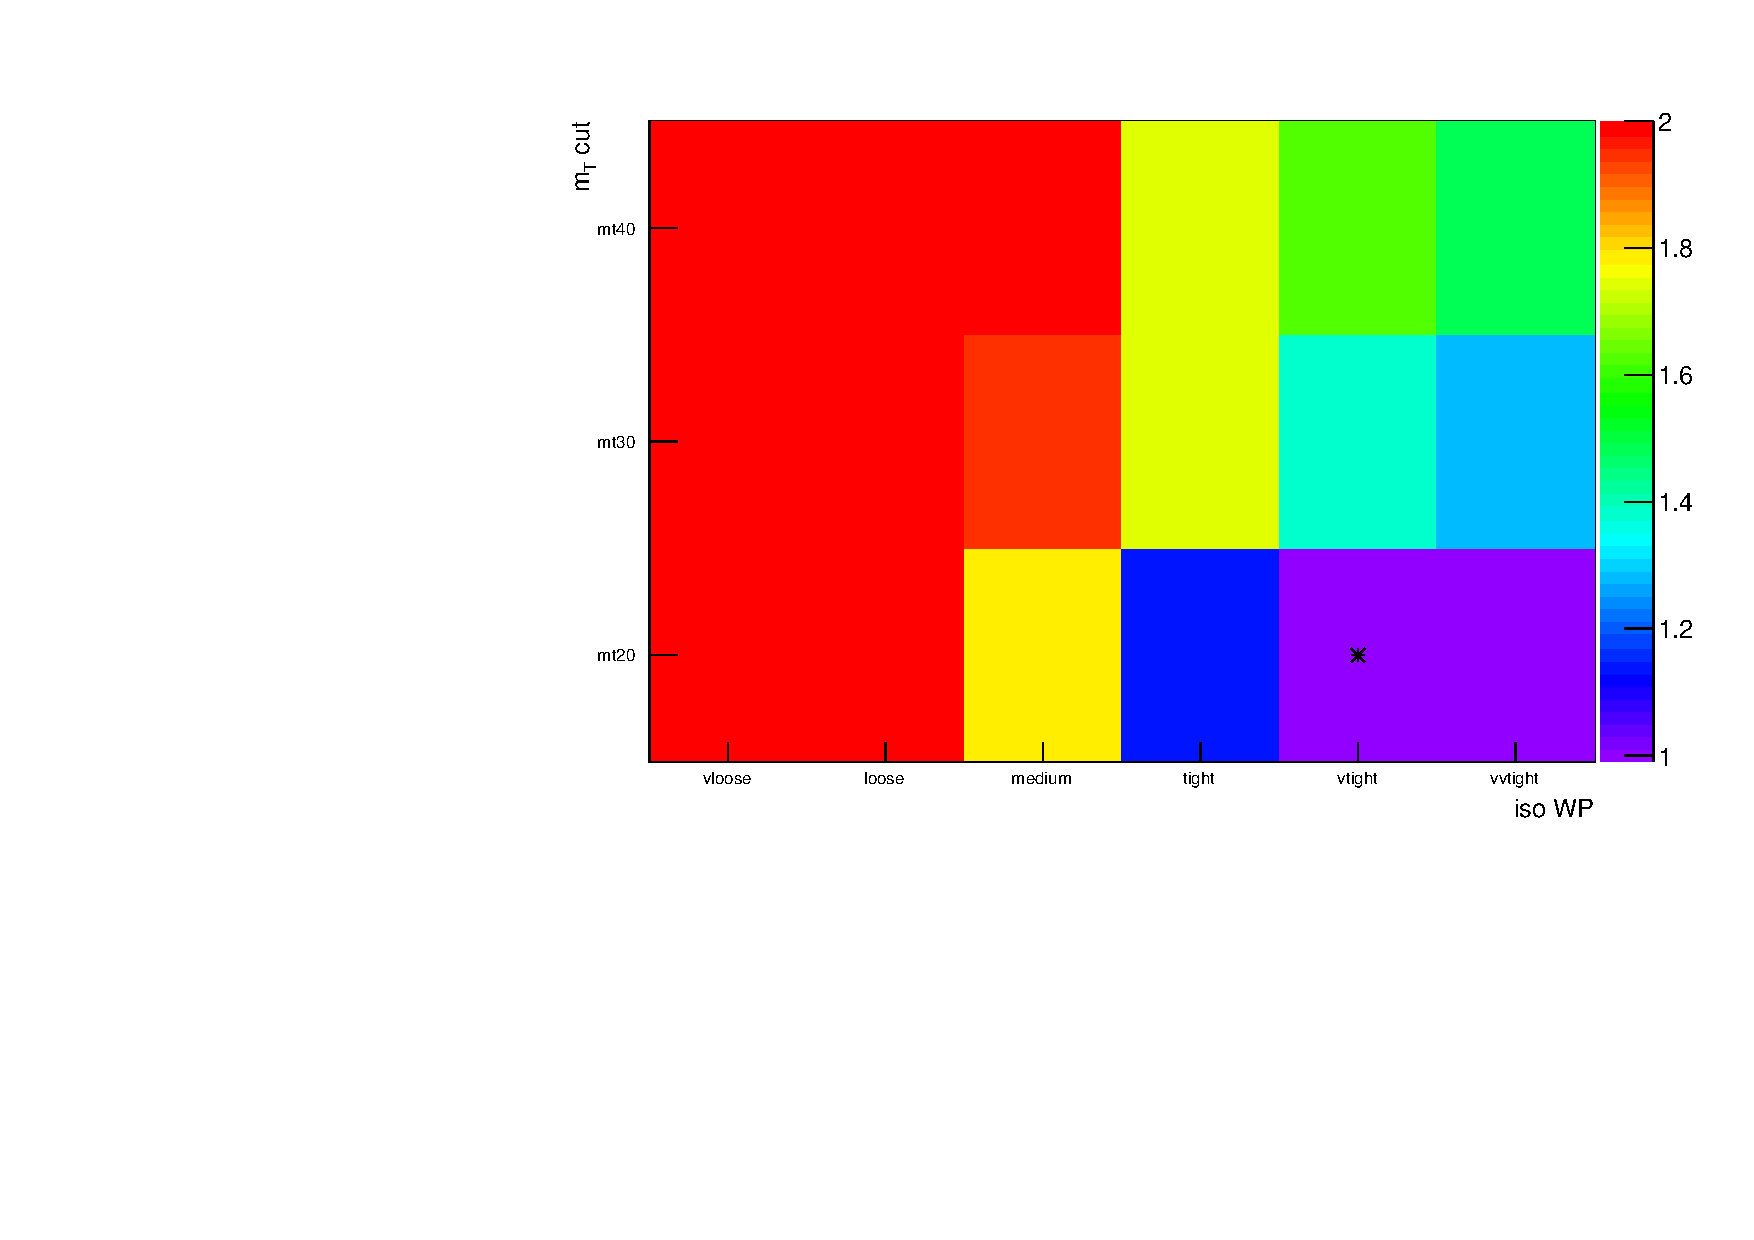
\includegraphics[width=0.5\textwidth]{./MSSM/Figures/optimisation_ggh_mt_160_range12.pdf}}
\subfloat[$m_{\phi} = 900$ GeV]{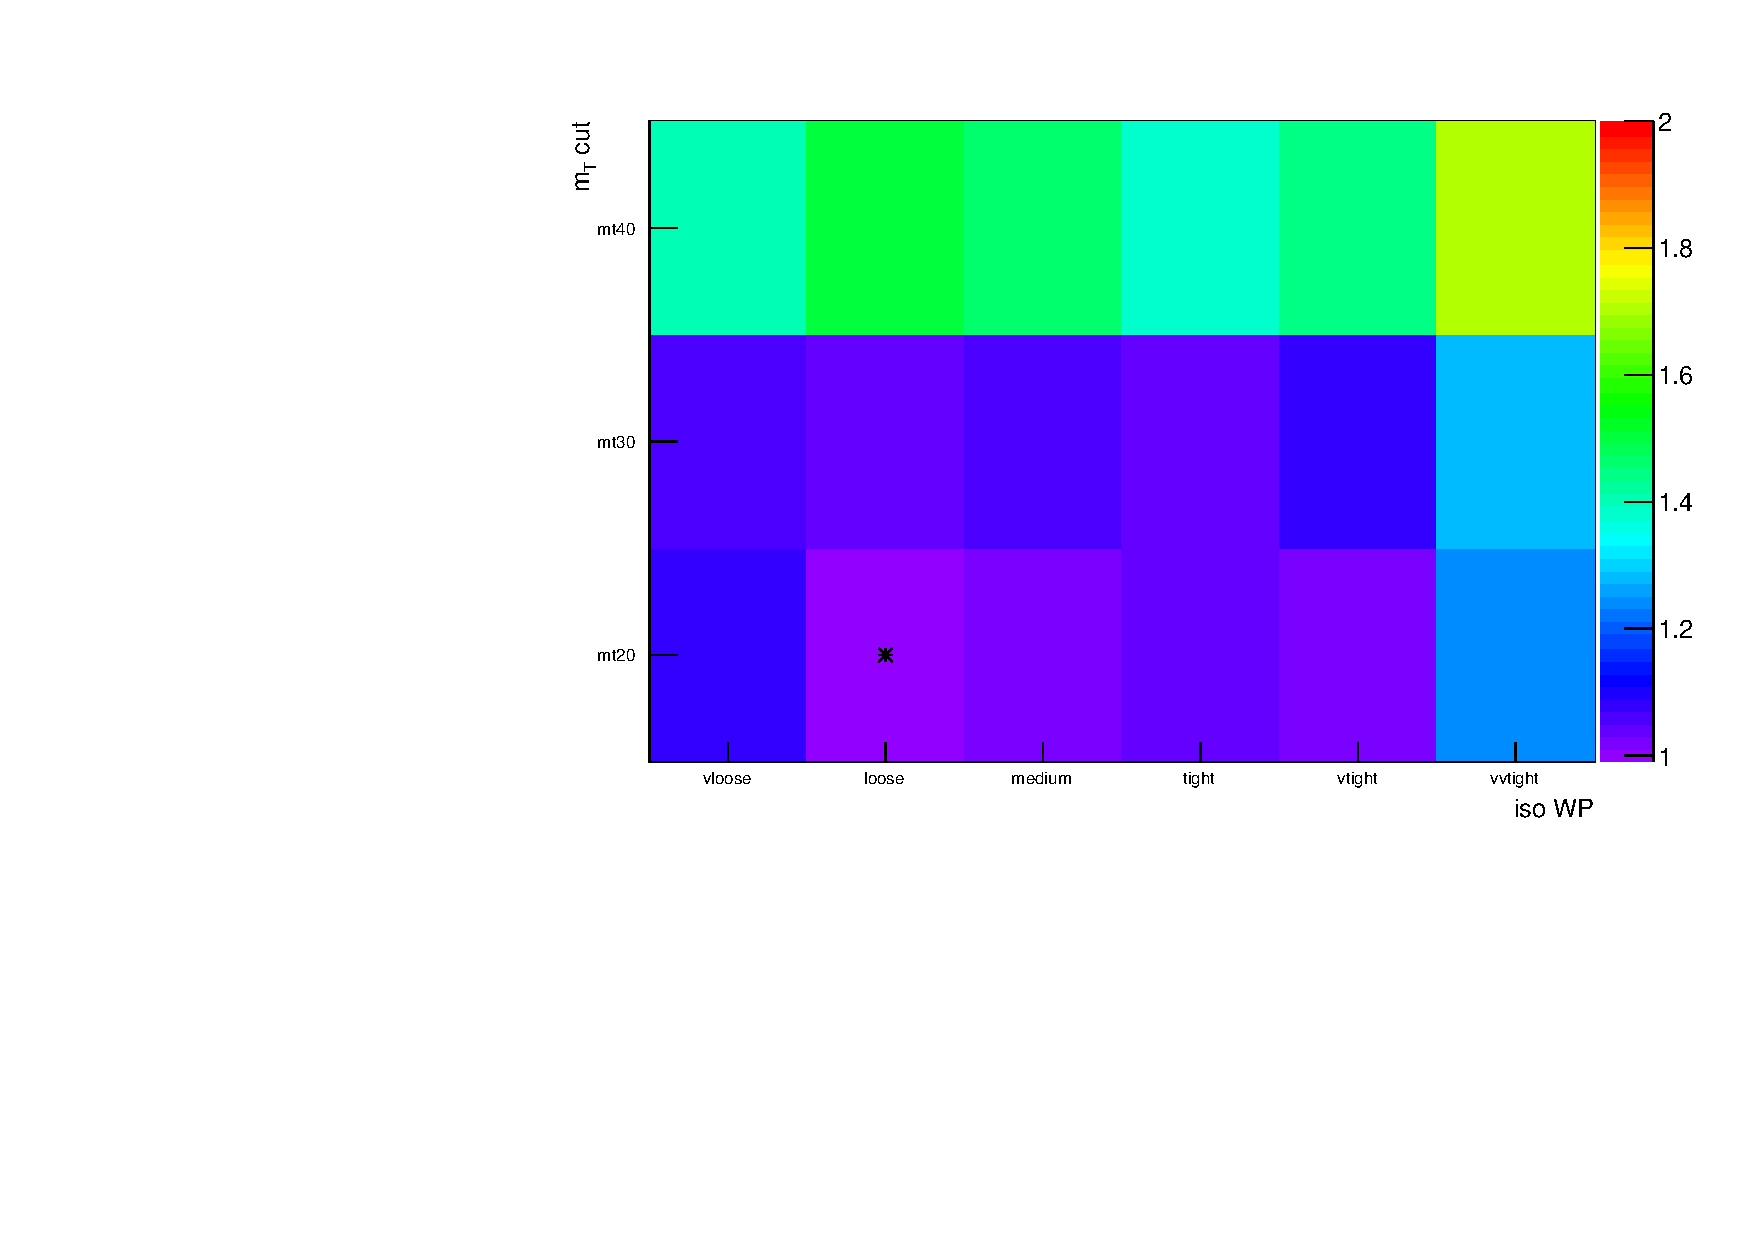
\includegraphics[width=0.5\textwidth]{./MSSM/Figures/optimisation_ggh_mt_900_range12.pdf}}~\\
\subfloat[$m_{\phi} = 1600$ GeV]{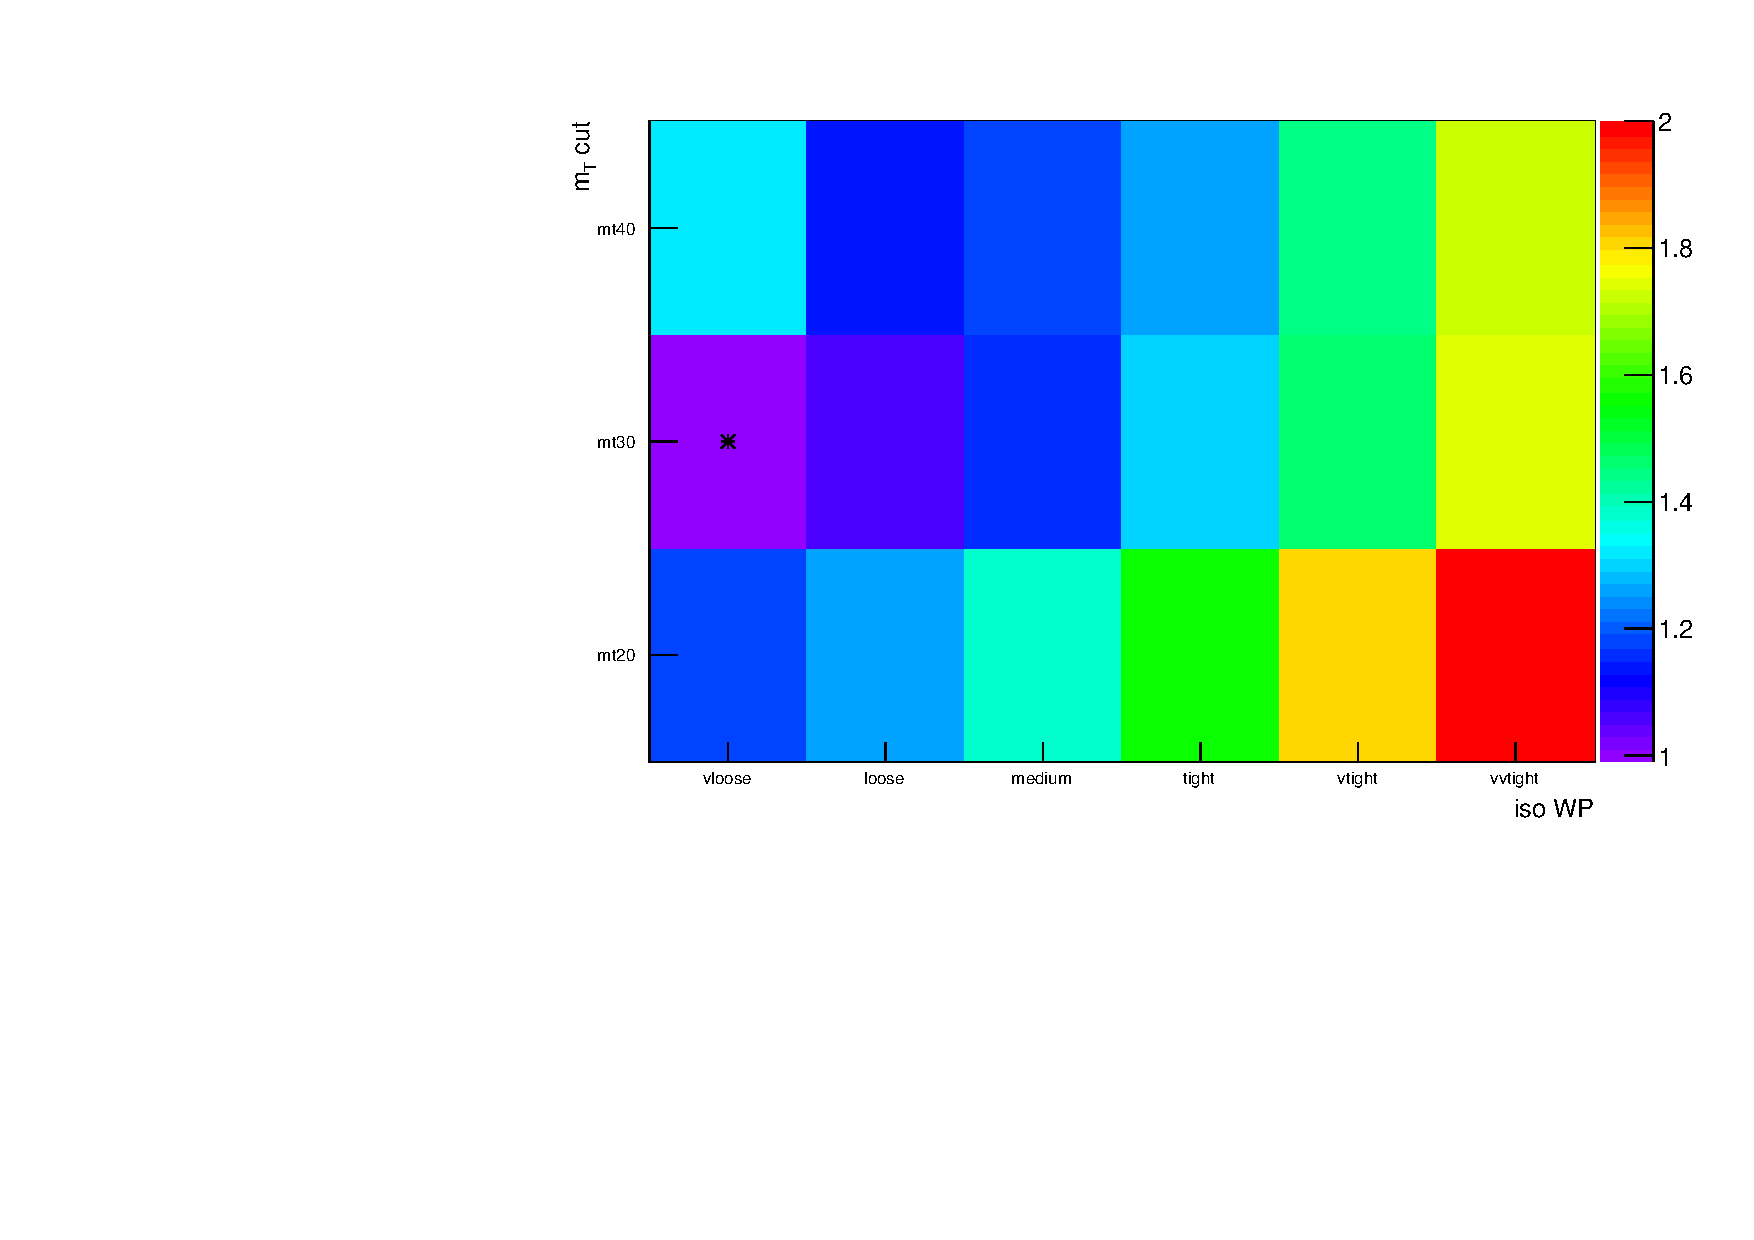
\includegraphics[width=0.5\textwidth]{./MSSM/Figures/optimisation_ggh_mt_1600_range12.pdf}}
\subfloat[$m_{\phi} = 2900$ GeV]{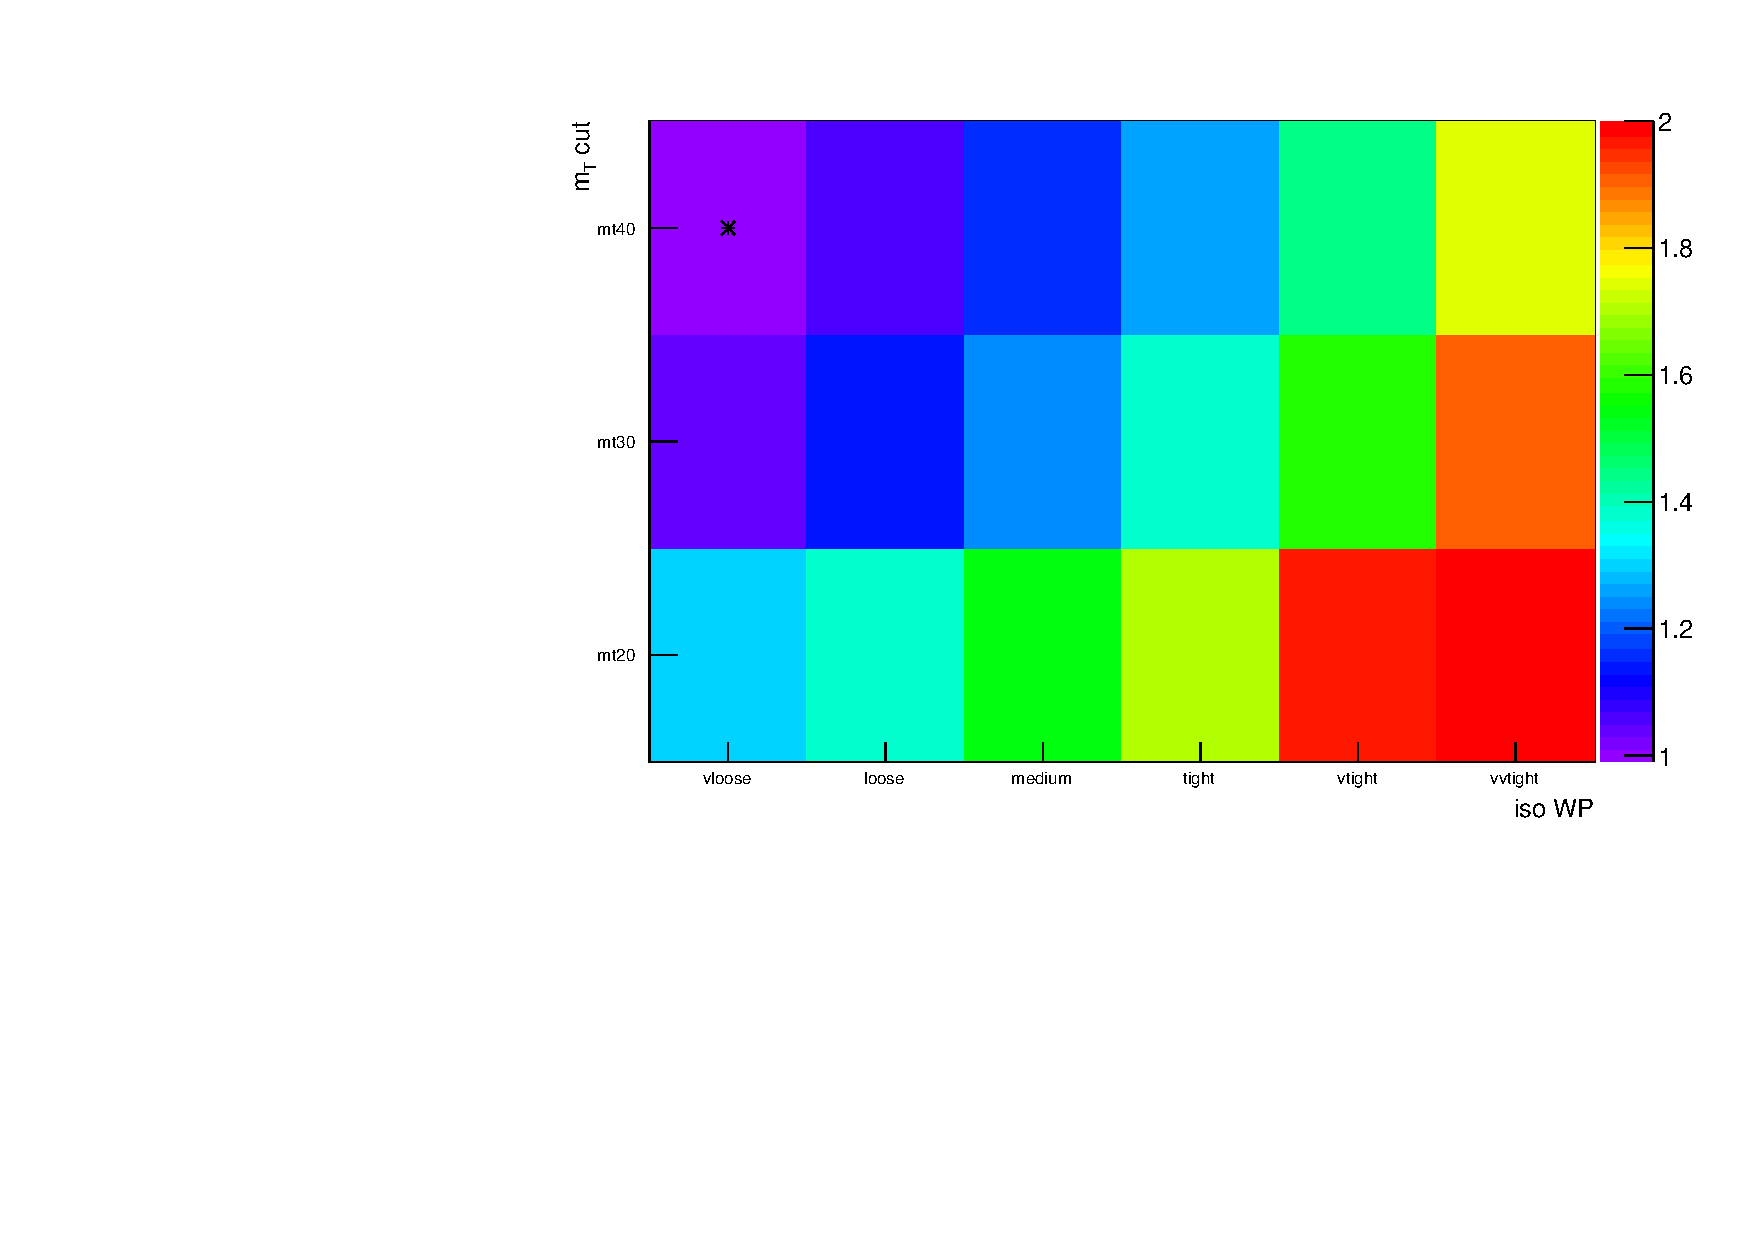
\includegraphics[width=0.5\textwidth]{./MSSM/Figures/optimisation_ggh_mt_2900_range12.pdf}}
\end{center}
\caption{Pre--fit expected limit on $\sigma\times$BR for the gg$\phi$ production process with decay into $\Pgt\Pgt$,
s a function of tau isolation working point (from very loose to very very tight) and
of \mT~ cut from \mT$<20$ GeV to \mT$<40$ GeV, normalised to the best limit in the plane, indicated by the asterisk. This is shown
for $m_{\phi}$ = 160 GeV (a), 900 GeV (b), 1600 GeV (c) and 2900 GeV (d). The most optimal combination of \mT~selection and 
hadronic tau isolation working point varies by mass point, with looser selections preferred for higher masses.}
\label{fig:mssm_selection_mt_taumt}.
\end{figure}

Based on this information, for the analysis on the 2015 dataset the selection was optimised
for mass points around 700-800 GeV. For the analysis on the 12.9 fb$^{-1}$ collected
in the first half of 2016, the selection was further loosened by 10 GeV in \mT~cut
and one step in hadronic tau isolation working point, to obtain the medium isolation working
point selection combined with a selection on \mT$<40$ GeV.

The choice of the hadronic tau \pT selection is driven by the effect on the low mass region:
raising the \pT selection by 10 GeV from the minimum of 20 GeV does not affect the sensivity
of the analysis for high mass points, while recovering some of the loss of loosening 
tau isolation working point and \mT~cut. The reason for this is that when using \pT$>30$ GeV 
fewer background events are selected. The effect of the increased hadronic tau \pT~ cut on the 
upper limits for the gg$\phi$ production process
in figure \ref{fig:mssm_tauptcut}a, and on the bb$\phi$ production process
in figure \ref{fig:mssm_tauptcut}b. At low mass the improvement in the gg$\phi$ limits
obtained by increasing the \pT~cut is sizeable, for bb$\phi$ events the effect is much
less pronounced.

\begin{figure}[h!]
\begin{center}
\subfloat[gg$\phi$]{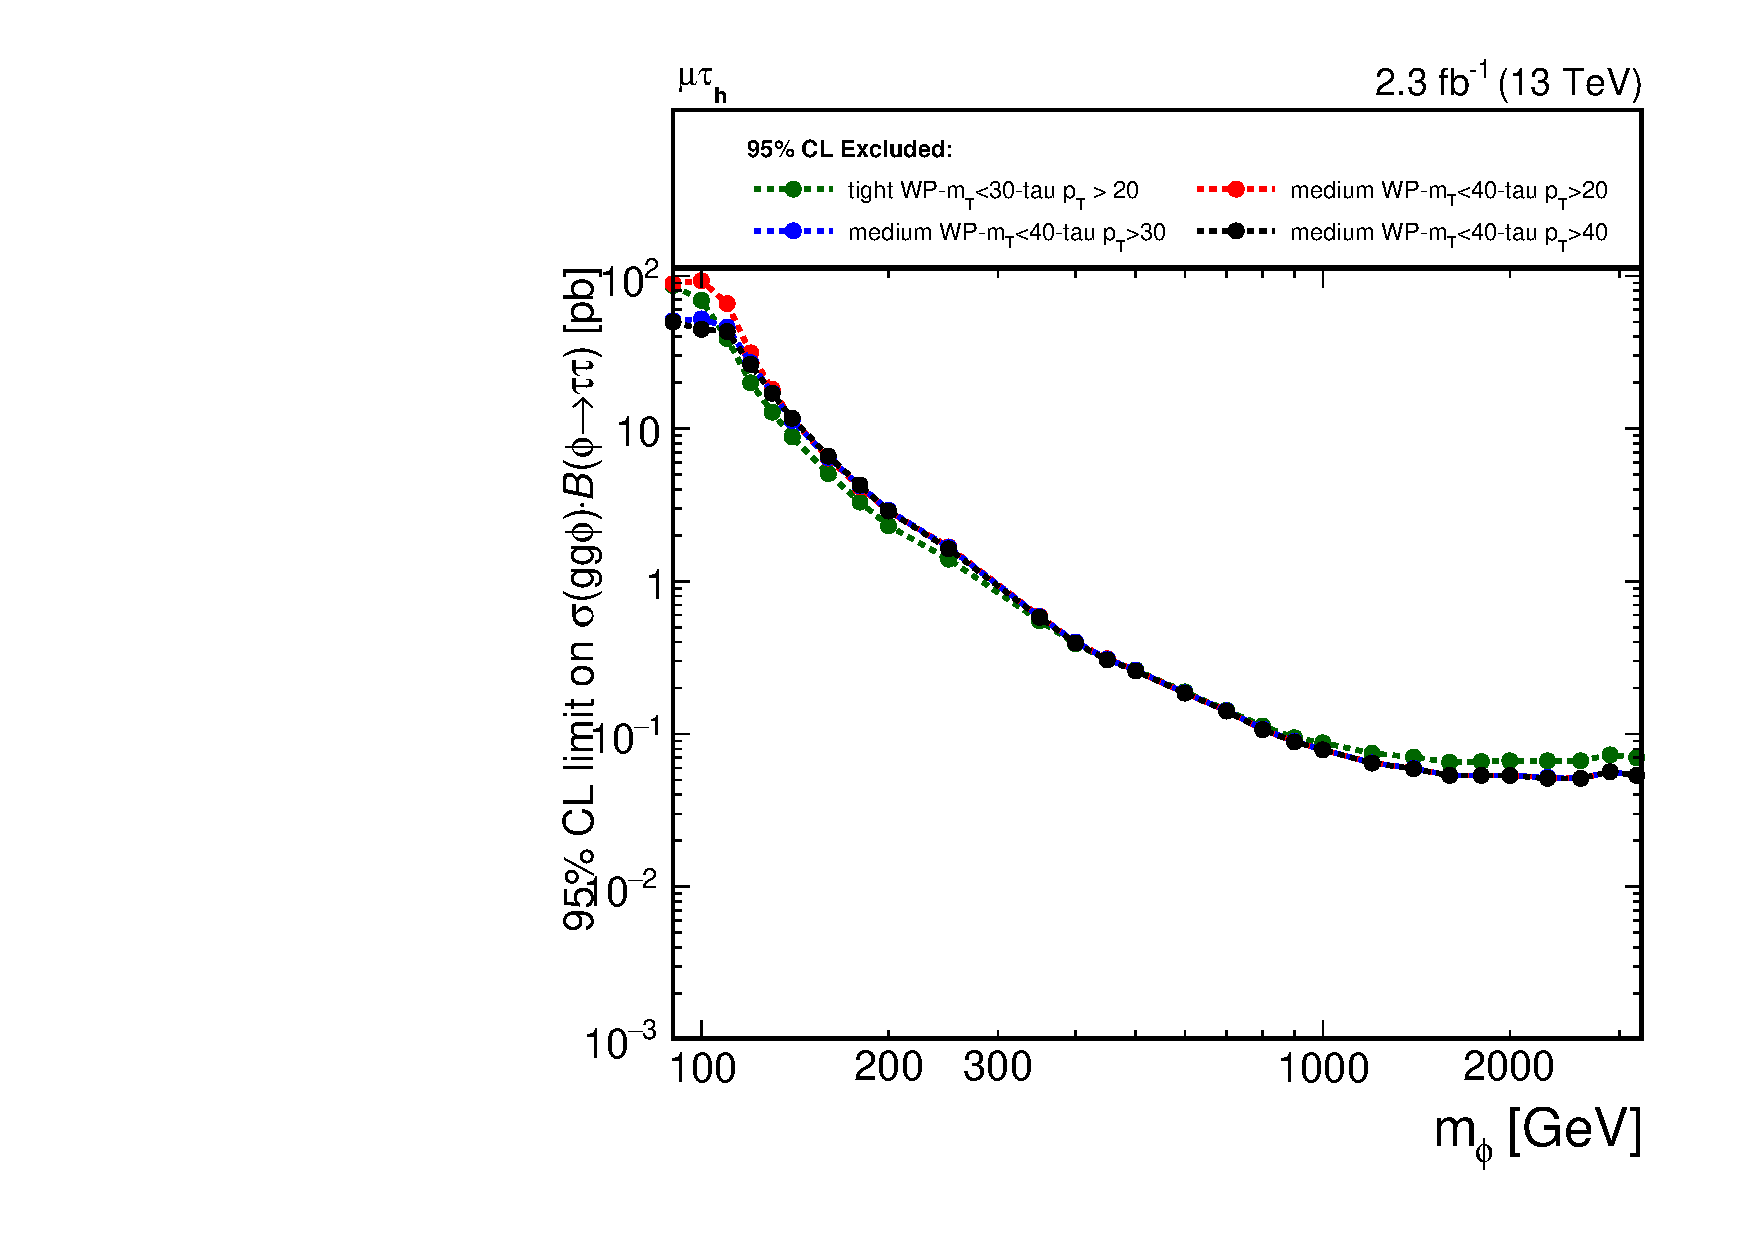
\includegraphics[width=0.5\textwidth]{./MSSM/Figures/mssm_optimisation_mediummt40_vs_tightmt30pt20_mt_ggH_remake.pdf}}
\subfloat[bb$\phi$]{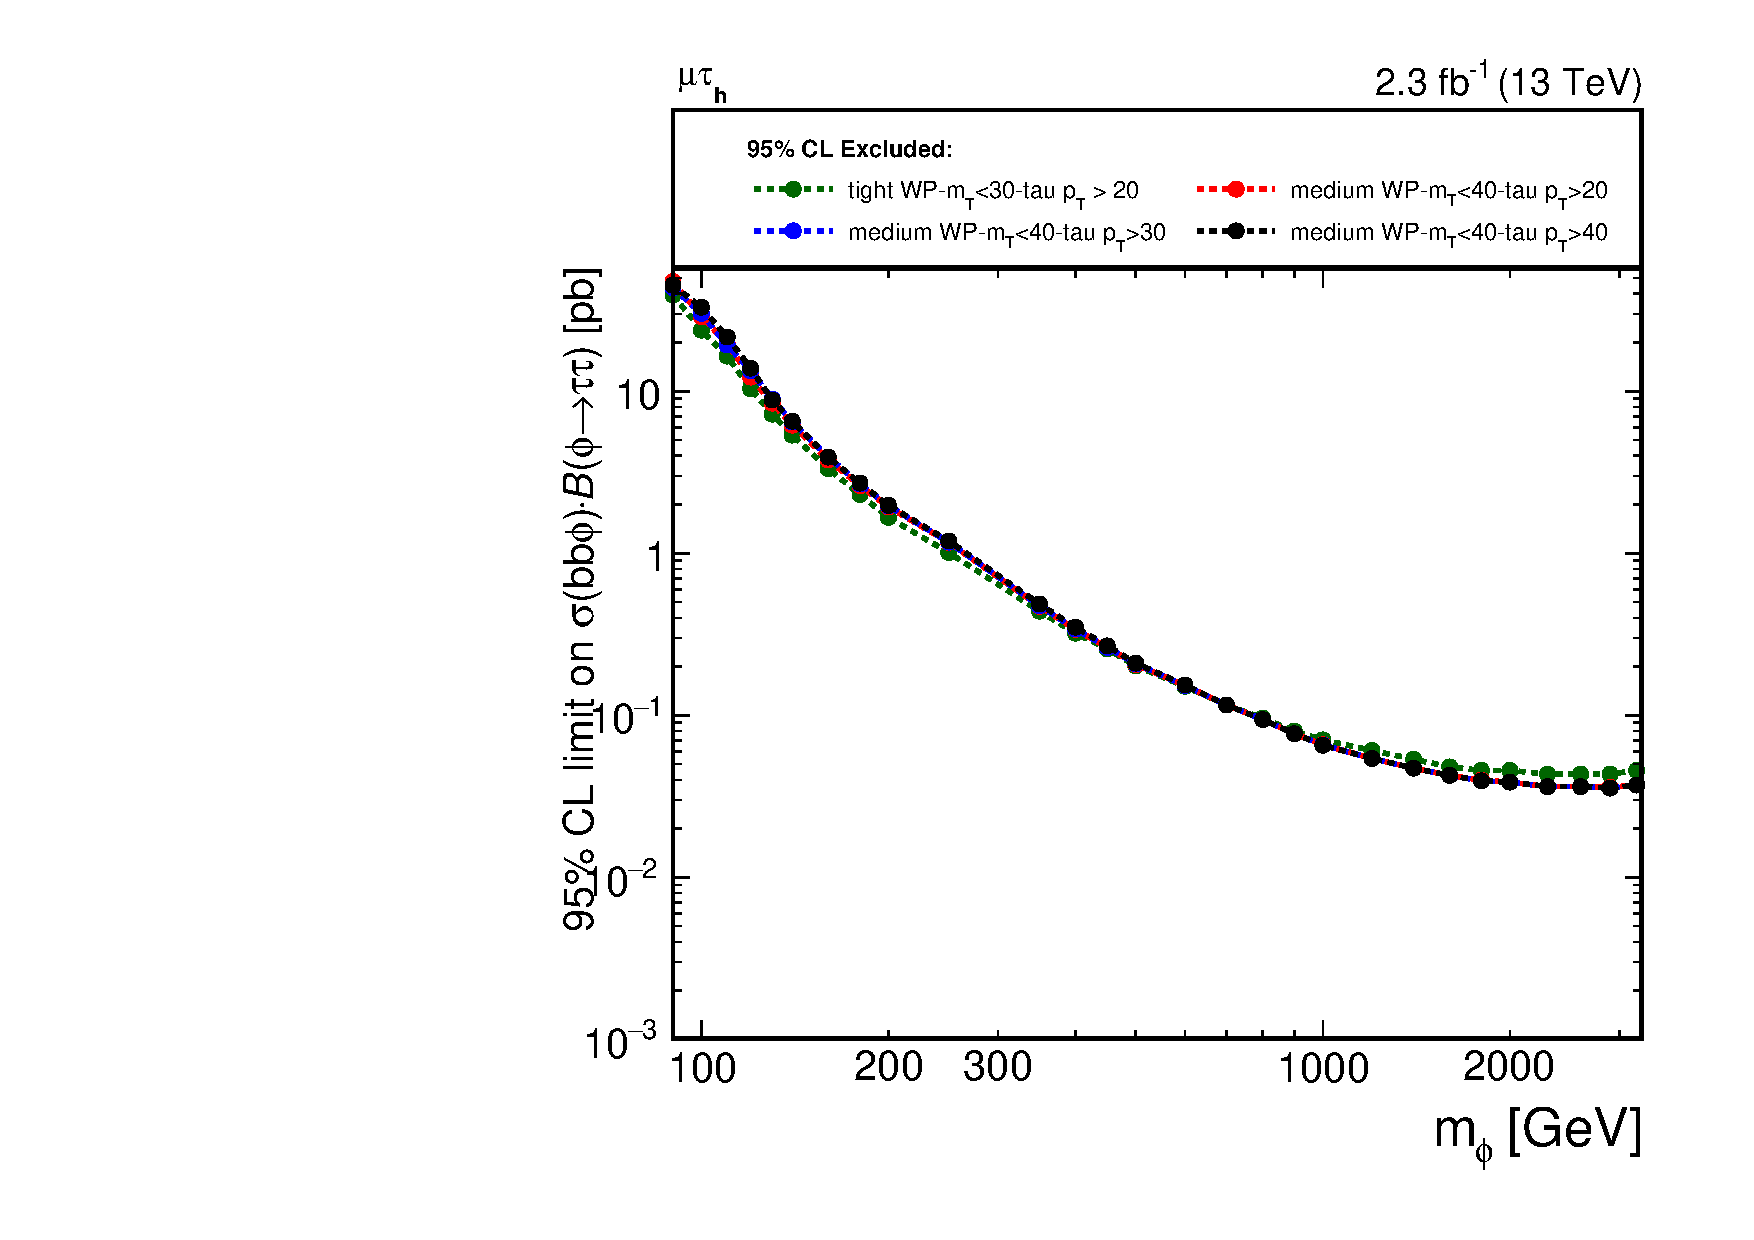
\includegraphics[width=0.5\textwidth]{./MSSM/Figures/mssm_optimisation_mediummt40_vs_tightmt30pt20_mt_bbH_remake.pdf}}
\end{center}
\caption{Pre-fit expected limits on $\sigma\times$BR in the \mutau channel for (a) gg$\phi$ production and (b) bb$\phi$ production. The
limits when using the medium hadronic tau isolation working point and \mT$<40$ GeV selection using a minimum
hadronic tau \pT~cut of 20 GeV (red circles), 30 GeV (blue circles) and 40 GeV (black circles) are shown. The green
circles show the limits using tighter tau isolation working point and \mT~selection. The limits on
the gg$\phi$ production process improve at low masses when increasing the hadronic tau \pT~cut,
the effect on the bb$\phi$ production process is less pronounced.}
\label{fig:mssm_tauptcut}
\end{figure}


\subsection{\texorpdfstring{Event selection in the \etau channel}{Event selection in the e tau channel}}
\label{sec:mssm_eventsel_et}
For selection of events in the \etau channel, the first step is
a trigger that only requires an electron at \ac{L1}. At the \ac{HLT}
loose identification and isolation criteria are then required.

The offline event selection proceeds to require an oppositely charged
electron and hadronically decaying tau, which are well--separated ($\Delta R > 0.5$).
The minimum \pT of the electron is required to be 26 GeV, with $|\eta| < 2.1$. %due to trigger conditions
This electron has to be consistent with having originated from the primary vertex, which
is achieved by requiring impact parameters $d_{xy} < 0.045$ cm and $d_{z} < 0.2$ cm, and it
is required to pass additional identification criteria. A selection on the MVA identification, which
selects electrons from \Zee events with 80\% efficiency, is used. In addition the
electron needs to be isolated. The relative isolation, calculated with a cone size of 0.3, is required to be $< 0.1$.

The hadronic tau is required to have a \pT greater than 30 GeV, $|\eta|<2.3$,
and is required to be reconstructed by the HPS algorithm and to pass the medium
working point of the MVA isolation discriminator. It also needs
to have originiated from the primary vertex and so the impact paramter $d_{z}$ is 
required to be less than 0.2 cm. Finally, the hadronic tau should
pass the tight working point of the anti--electron discriminator
and the loose working point of the anti--muon discriminator.

Just like for muons, it was found that the analysis is not highly sensitive
to the choice of electron isolation variable and selection, yet an effort
is made not to use a suboptimal selection.
A topological selection on the \mT~ variable is also made in this channel to reject \Wjets events. 
The used value of \mT $< 50$ is obtained by performing a 2D optimisation where the \mT~ selection
and hadronic tau isolation working point are varied at the same time. The same considerations as
for the \mutau channel apply. The choice of the hadronic tau \pT~ selection to 30 GeV is
chosen to recover some of the sensitivity lost at low mass by using looser \mT~ and hadronic
tau isolation selections. This is illustrated in figure \ref{fig:mssm_tauptcut_et}.

\begin{figure}[h!]
\begin{center}
\subfloat[gg$\phi$]{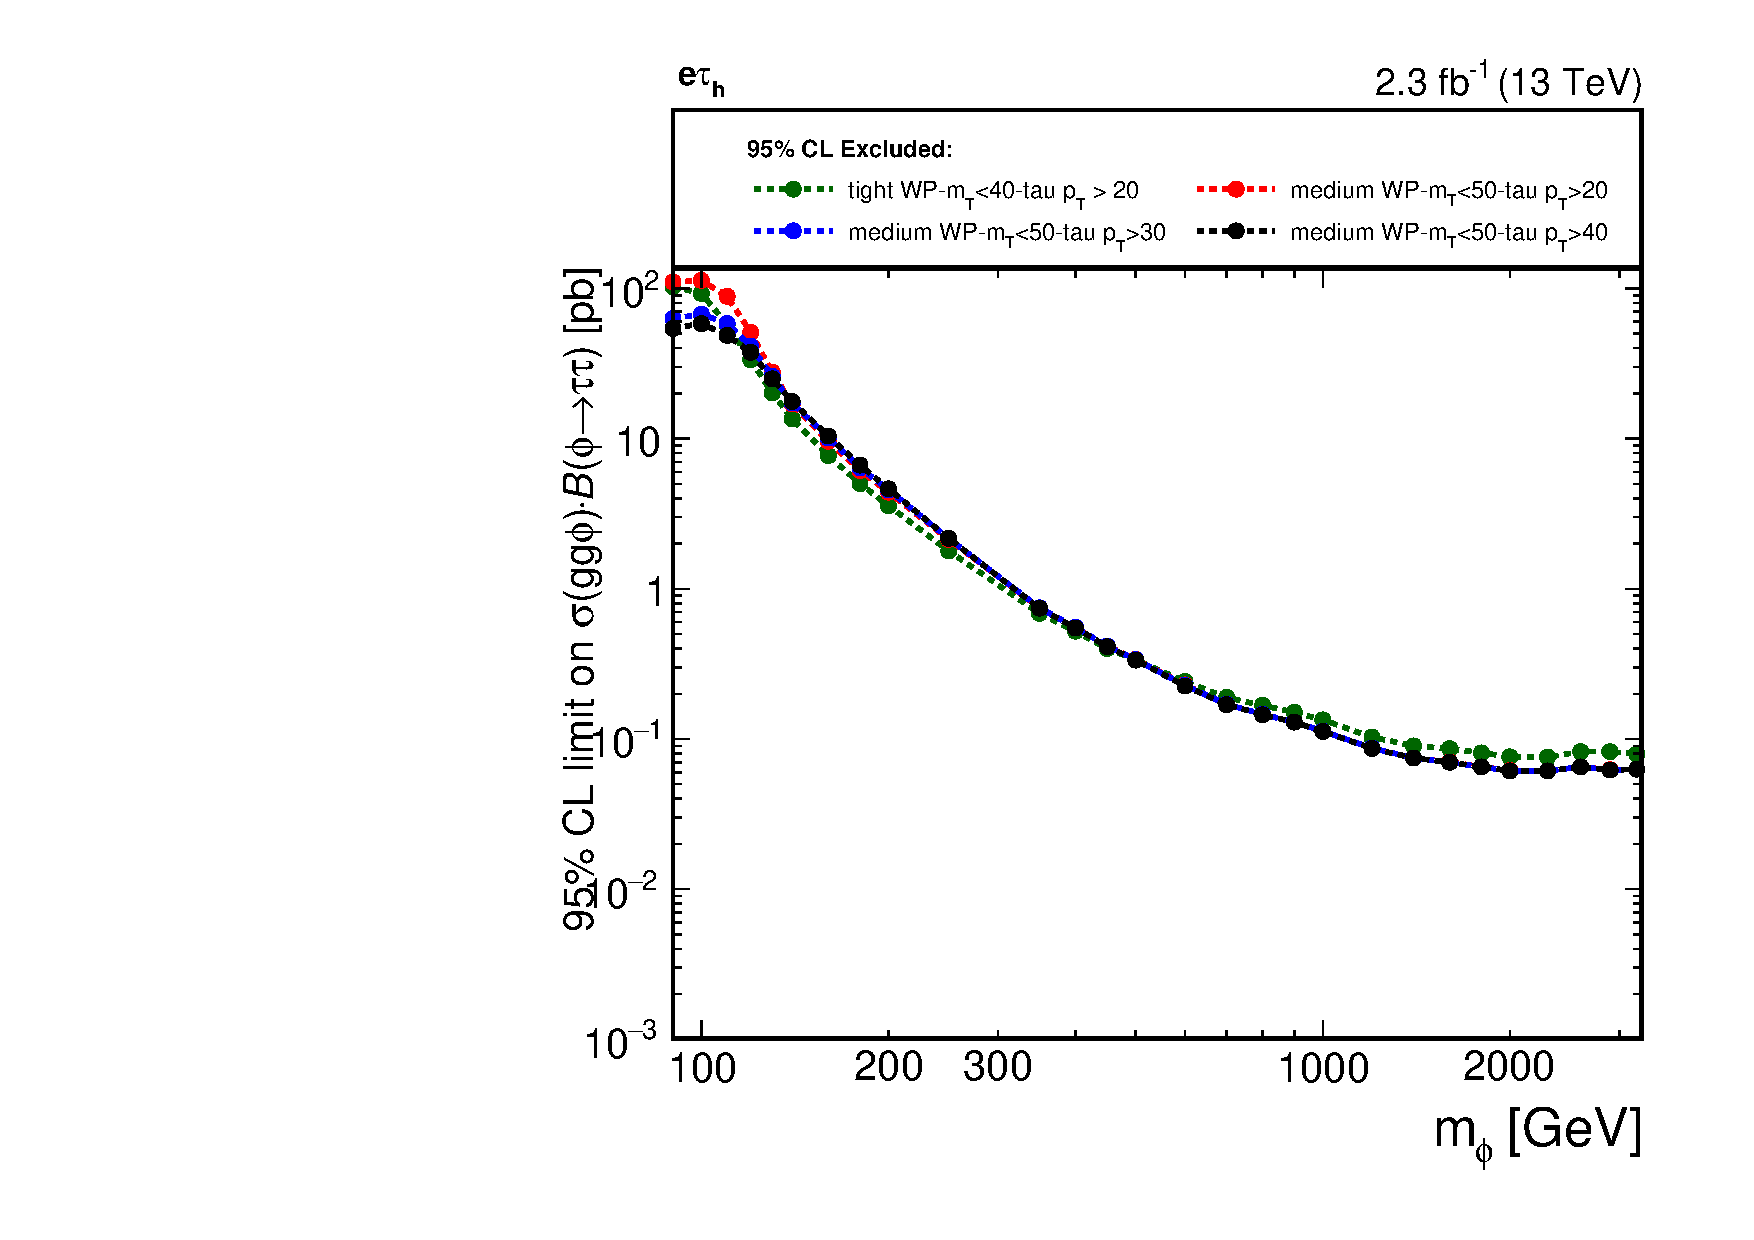
\includegraphics[width=0.5\textwidth]{./MSSM/Figures/mssm_optimisation_mediummt50_vs_tightmt40pt20_et_ggH_remake.pdf}}
\subfloat[bb$\phi$]{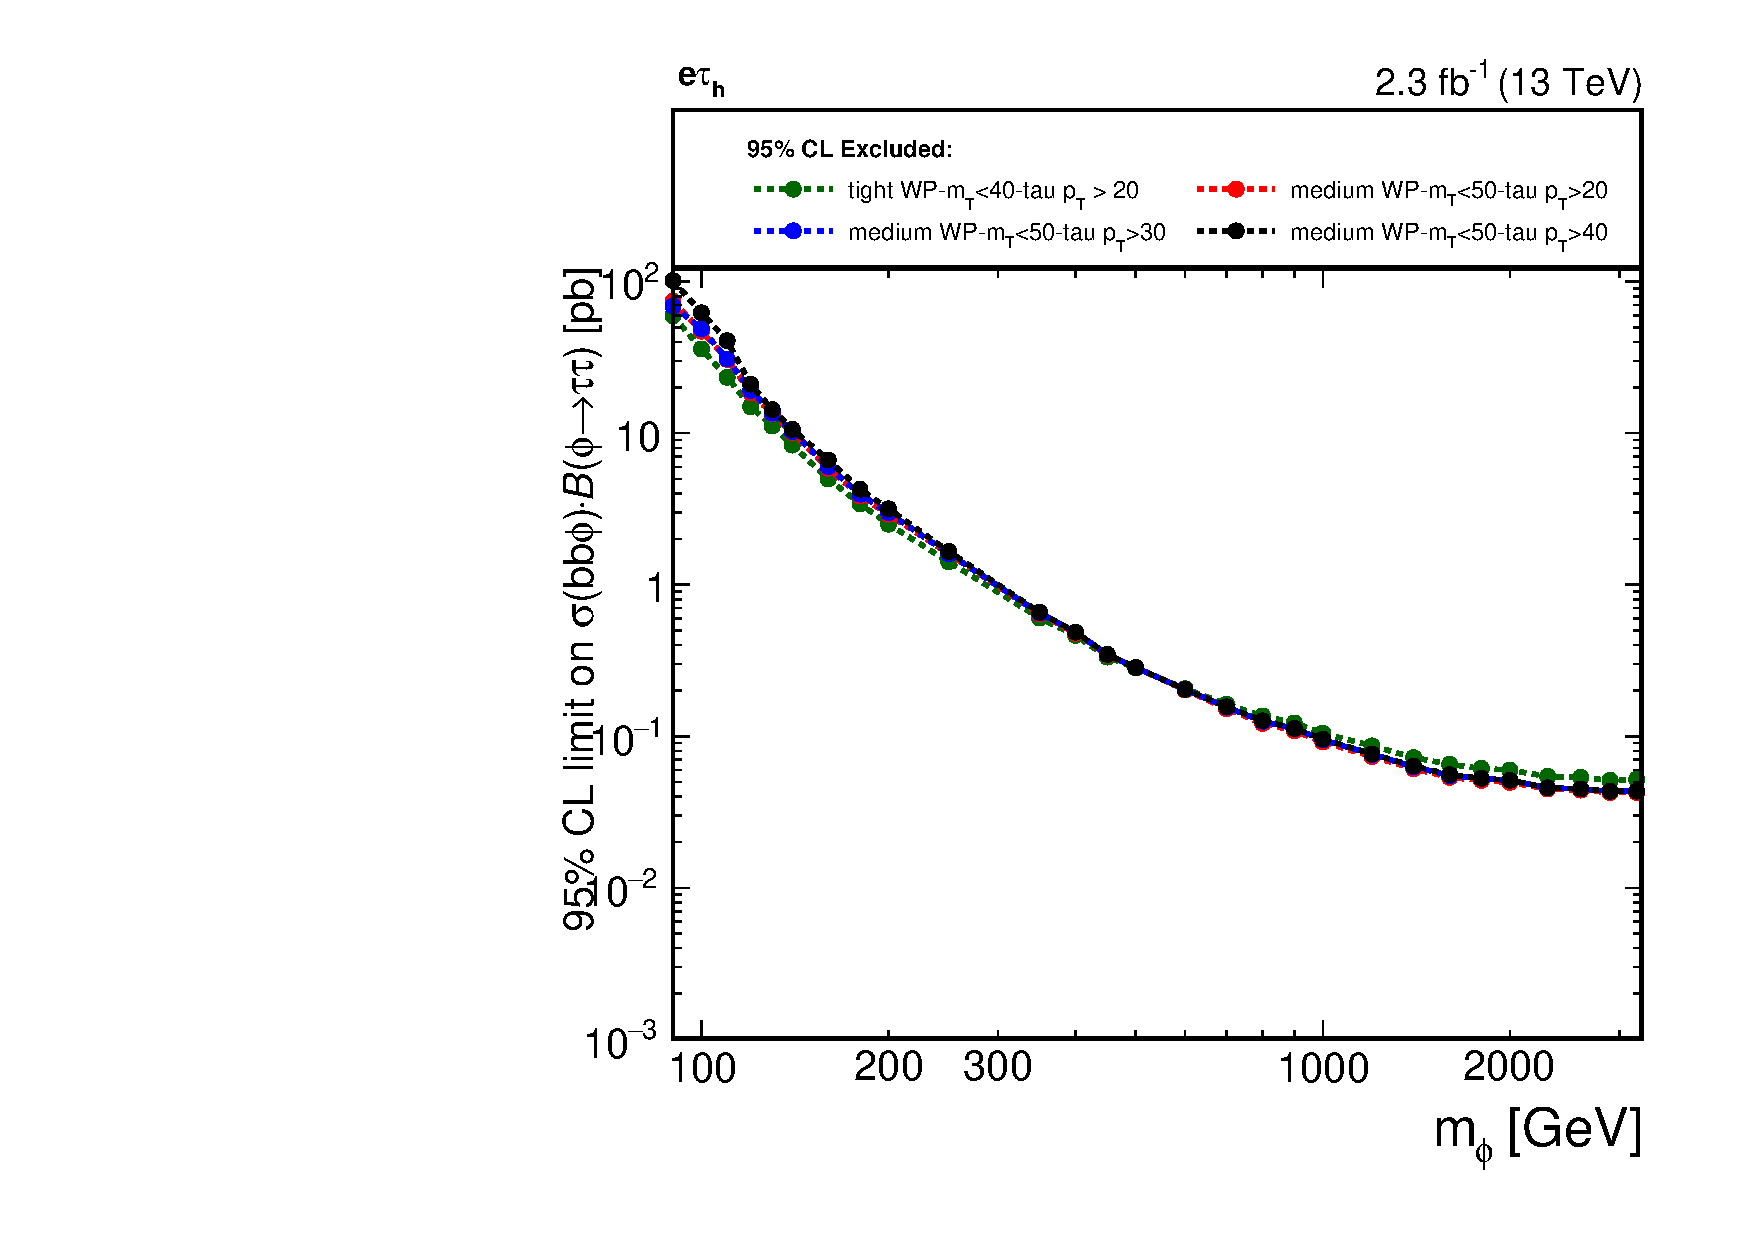
\includegraphics[width=0.5\textwidth]{./MSSM/Figures/mssm_optimisation_mediummt50_vs_tightmt40pt20_et_bbH_remake.pdf}}
\end{center}
\caption{Pre-fit expected limits on $\sigma\times$BR in the \etau channel for (a) gg$\phi$ production and (b) bb$\phi$ production. The
limits using the medium hadronic tau isolation working point and \mT$<40$ GeV selection using a minimum
hadronic tau \pT~cut of 20 GeV (red circles), 30 GeV (blue circles) and 40 GeV (black circles) are shown. The green
circles show the limits using tighter tau isolation working point and \mT~selection. The limits on
the gg$\phi$ production process improve at low masses when increasing the hadronic tau \pT~cut,
the effect on the bb$\phi$ production process is less pronounced.}
\label{fig:mssm_tauptcut_et}
\end{figure}


\subsection{\texorpdfstring{Event selection in the \tautau channel}{Event selection in the tau tau channel}}
\label{sec:mssm_eventsel_tt}
Selection of events in the \tautau channel starts with a trigger
that requires two hadronic taus at \ac{L1}. At the level of the \ac{HLT}, loose identification
and isolation criteria are applied to these hadronic taus.

The offline event selection continues by requiring both hadronic taus to be oppositely charged, separated
by $\Delta R > 0.5$, have pT~ of at least 40 GeV and $|\eta|<2.1$. Both taus need
to pass decay mode finding and have originated from the primary vertex, with the impact parameter $d_{z} < 0.2$ cm. 
Both taus need to pass the tight working point of the isolation discriminator, the very loose 
working point of the anti--electron discriminator and the loose working point of the anti--muon discriminator. 
The tight working point of the isolation discriminator is chosen to optimise the sensitivity
of this channel for higher masses. INSERT PLOT

\subsection{\texorpdfstring{Event selection in the \emu channel}{Event selection in the e mu channel}}
\label{sec:mssm_eventsel_em}
Events in the \emu channel are first selected by two triggers
that both require an electron and muon at \ac{L1} and apply loose ID and
isolation requirements to these objects at \ac{HLT}. The \pT requirements on
the electron and muon are different in the two triggers, thus using the combination of the two
improves the analysis performance.

The offline requirements to the \emu pair are that the electron 
and muon are oppositely charged, separated by $\Delta R >$ 0.3. The 
electron should have a minimum \pT~ of 13 GeV and have $|\eta|< 2.5$. As
in the \etau channel the electron's impact parameters have to 
satisfy $d_{xy} < 0.045$ cm and $d_{z}<0.2$ cm. A selection is
made on the electron identification MVA, using a working point that 
is 80\% efficient for electrons in \Zee decays. The electron
also needs to be isolated, with the relative isolation calculated
with a cone size of 0.3 being less than $<0.15$.

The muons need to have a \pT~of at least 10 GeV, $|\eta|<2.4$ and 
their impact parameters need to be $d_{xy}<0.045$ cm and $d_{z}<0.2$ cm.
In addition to the kinematic requirements the muon must
pass the medium identification criteria and be isolated with the relative
isolation, calculated with a cone size of 0.4, required to be less than 0.15.

Because a combination of triggers is used, the object firing
the higher \pT~ trigger leg needs to have a transverse momentum
of at least 24 GeV on top of the requirements already discussed.
In addition, a topological selection is made on the $D_{\zeta}$ variable \cite{cdf-dzeta},
\begin{align}\label{eqn:mssm_em_dzeta}
D_{\zeta} = P_{\zeta} - 1.85 P_{\zeta}^{\text{vis}}, \notag \\
\text{where } P_{\zeta} = (\vec{p}_{\text{T},1}^{\text{vis}} + \vec{p}_{\text{T},2}^{\text{vis}} + E_{\text{T}}^{\text{miss}})\frac{\vec{\zeta}}{|\vec{\zeta}|}, \notag \\
\text{and } P_{\zeta}^{\text{vis}} = (\vec{p}_{\text{T},1}^{\text{vis}}+\vec{p}_{\text{T},2}^{\text{vis}})\frac{\vec{\zeta}}{|\vec{\zeta}|}.
\end{align}

Thus $D_{\zeta}$ is the difference of the projection of the visible tau decay products plus missing energy \pT+\MET,
and simply the visible tau decay product \pT on the axis $\vec{\zeta}$. This is the axis that bisects 
the directions $\vec{p}_{\text{T,1}}^{\text{vis}}$ and $\vec{p}_{\text{T,2}}^{\text{vis}}$
of the visible decay products in the transverse plane. This selection is illustrated in figure
\ref{fig:mssm_dzeta}a, with figure \ref{fig:mssm_dzeta}b showing the $D_{\zeta}$ distribution
for \emu events. The used cut value, $D_{\zeta} > -20$ GeV rejects $\ttbar$, \Wjets and diboson
events. 
%The momentum of the neutrinos should not be in the opposite direction of the sum of the visible decay products
%as the neutrinos and visible tau decay products travel at small angles from the original tau.

\begin{figure}[h!]
\begin{center}
\subfloat[Reconstruction of $D_{\zeta}$]{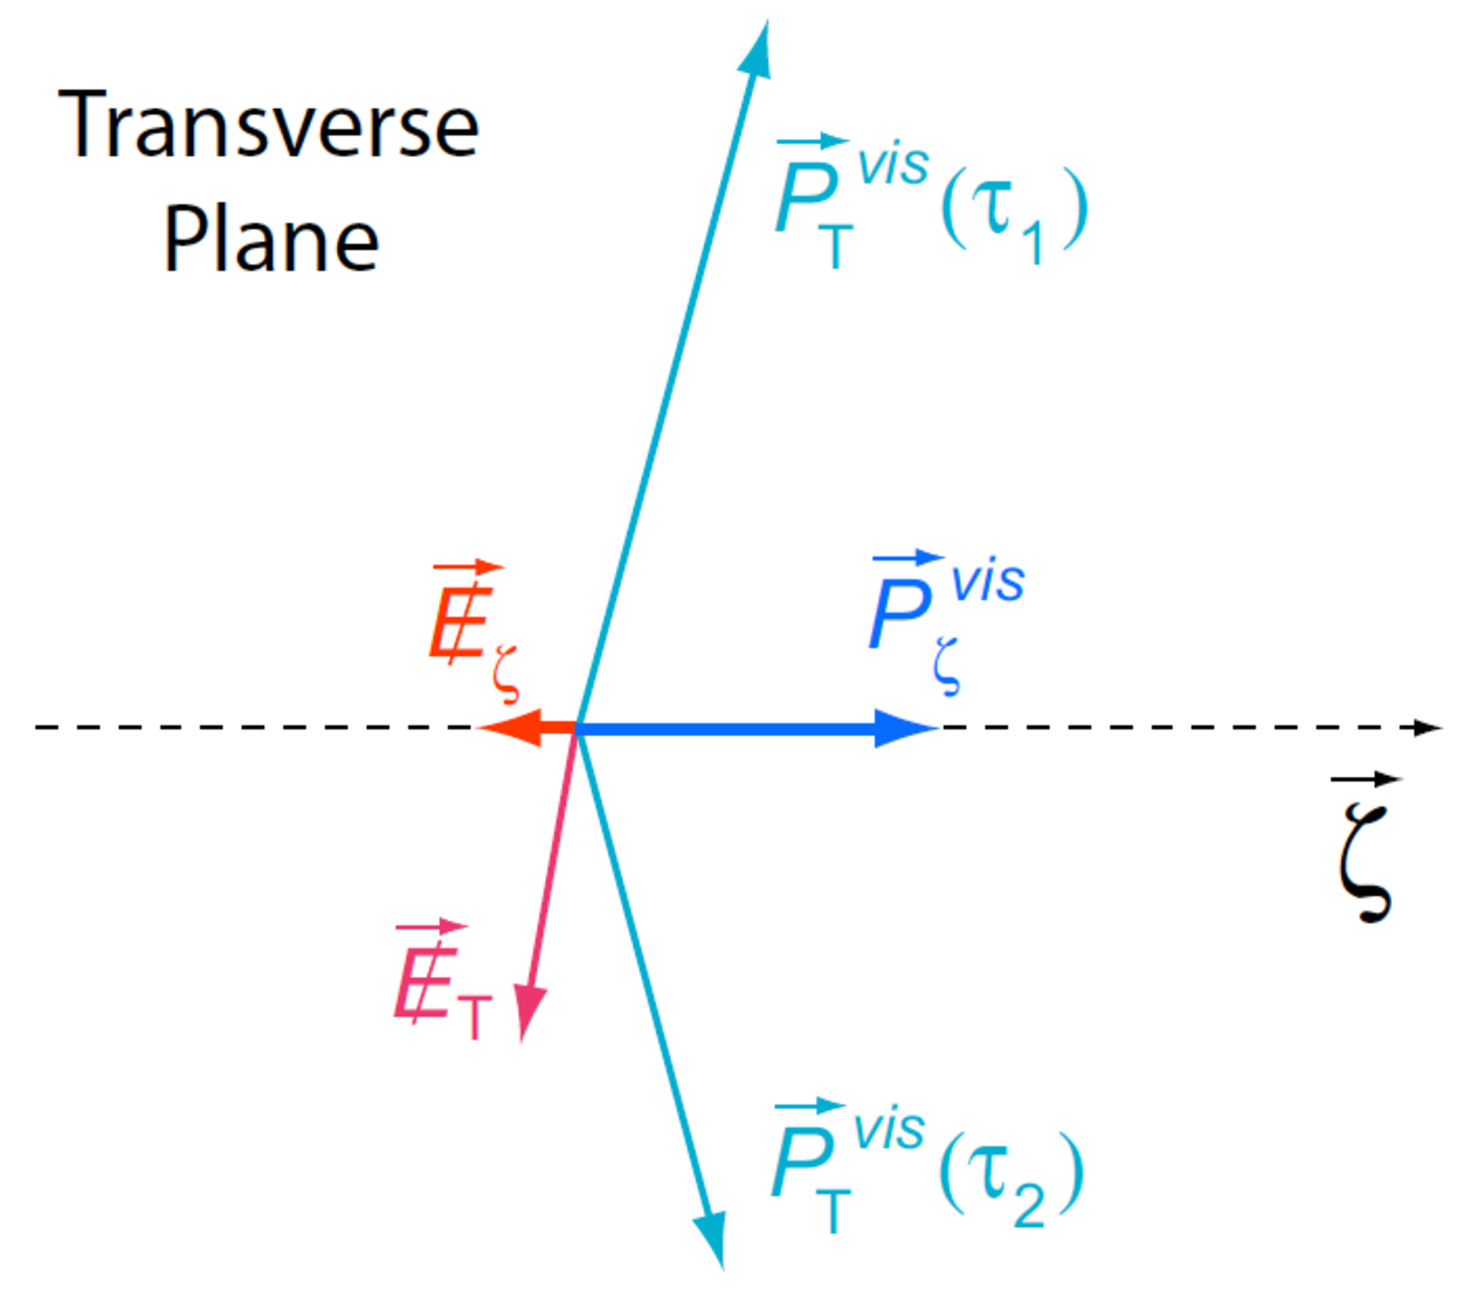
\includegraphics[width=0.5\textwidth]{./MSSM/Figures/PZeta.pdf}}
\subfloat[$D_{\zeta}$ distribution in \emu channel]{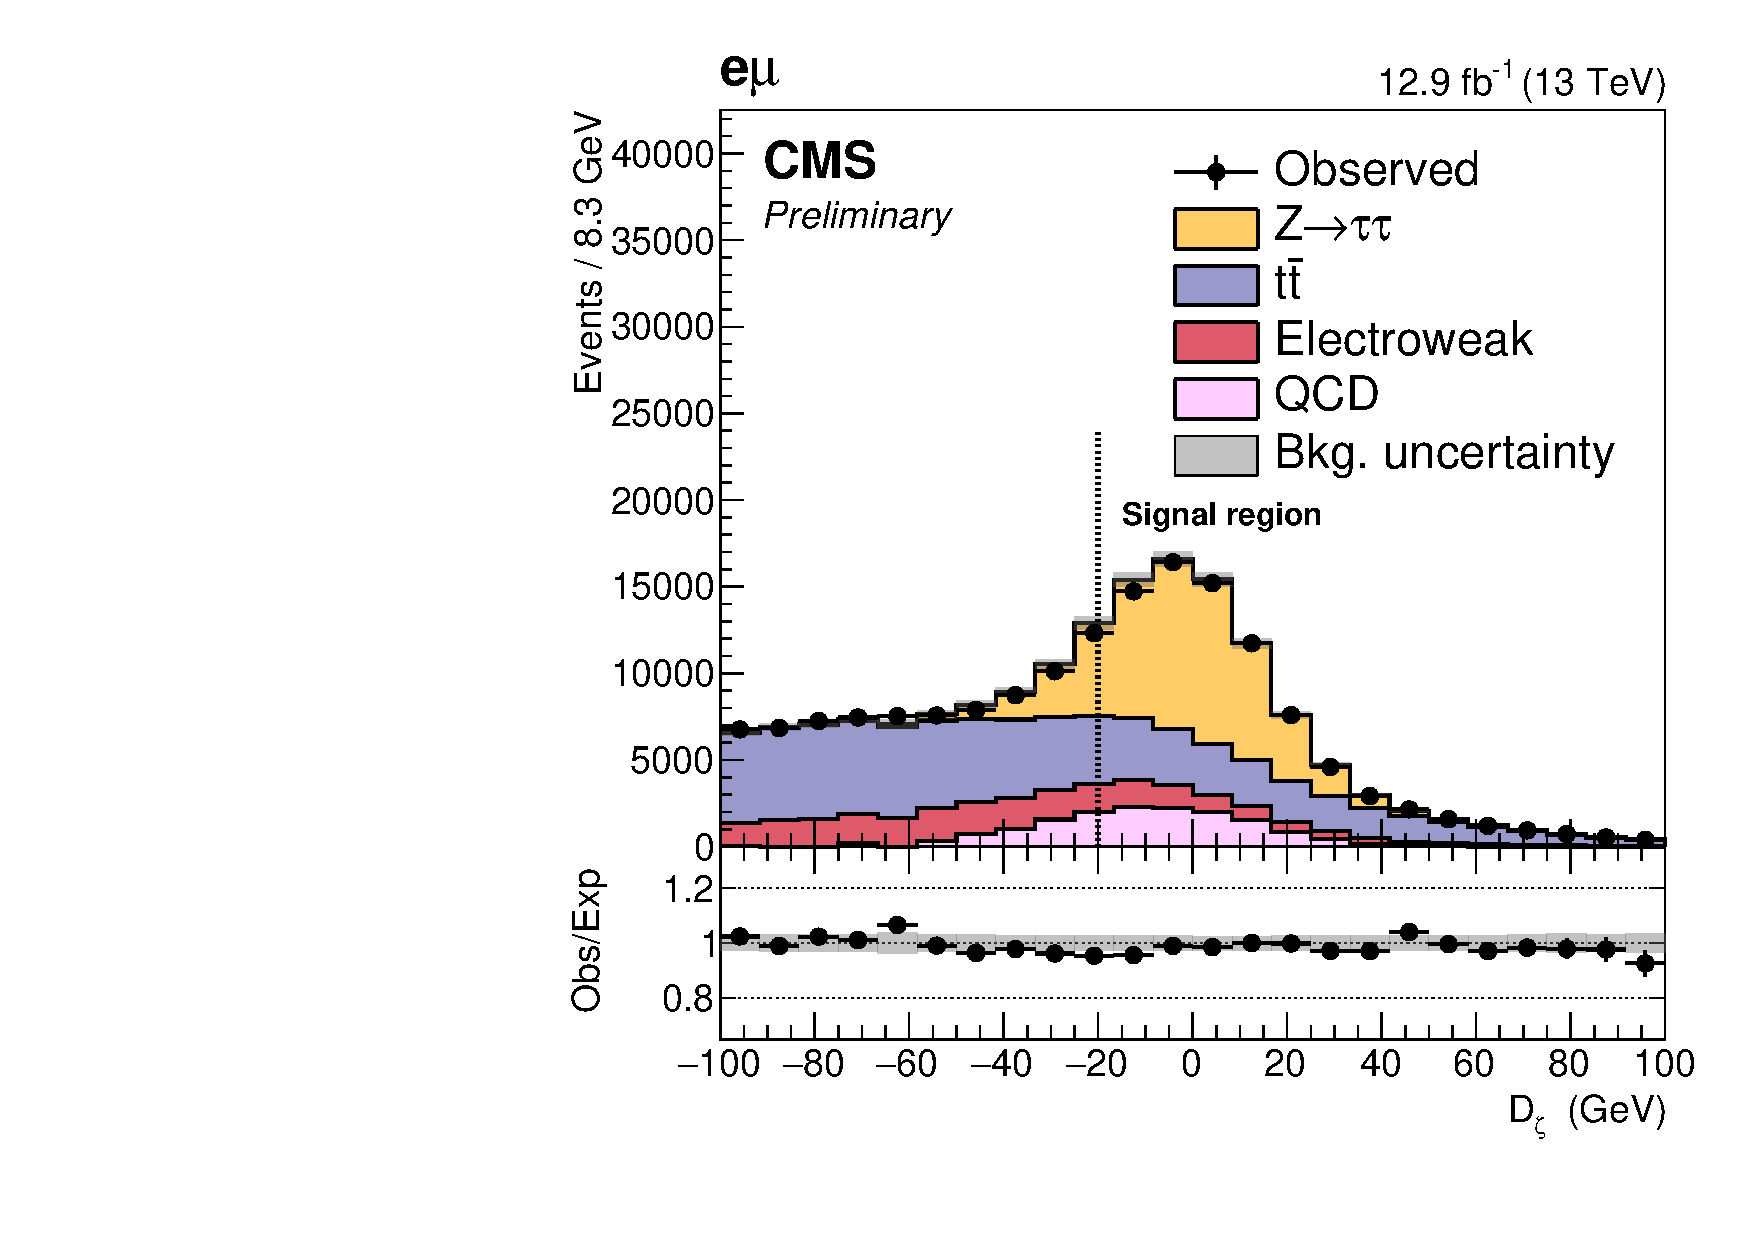
\includegraphics[width=0.5\textwidth]{./MSSM/Figures/pzeta_inclusive_em_2016.pdf}}
\end{center}
\caption{(a) reconstruction of $D_{\zeta}$ \cite{cdf-dzeta} and (b) $D_{\zeta}$ distribution in the 
\emu channel\cite{CMS-PAS-HIG-16-037}.}
\label{fig:mssm_dzeta}
\end{figure}


\subsection{Categorisation}
\label{sec:mssm_eventsel_categories}
As the analysis targets both the gluon--gluon fusion
and the b--associated production modes of MSSM Higgs
bosons, two exclusive categories are defined based on the 
number of b--tagged jets, where a jet is considered b--tagged
if it passes the medium working point of the \ac{CSV}v2 discriminator. 
\begin{itemize}
\setlength{\itemsep}{-\baselineskip}
\item \textbf{No b-tag}: 0 b--tagged jets. This category targets the gg$\phi$ production mode but is also sensitive to some of the bb$\phi$ signal
\item \textbf{b-tag}: At least 1 b--tagged jet and at most 1 
jet with \pT$>30$ GeV. Due to the different phase space considered for
b--tagging than for normal jet reconstruction this requirement does not necessarily
mean there will be only one jet in the event. The requirement reduces the sizeable \ttbar
background
\end{itemize}

Figure \ref{fig:mssm_cats_tt}a shows the number of jets 
in the \tautau channel, with \ref{fig:mssm_cats_tt}b showing
the number of b--tagged jets in that channel. The gluon--gluon fusion
signal and bb associated signal are overlaid on these distributions,
thus indicating the signal--sensitive bins, motivating the choice of categories.

\begin{figure}[h!]
\begin{center}
\subfloat[Number of jets]{\includegraphics[width=0.5\textwidth]{./MSSM/Figures/n_jets_inclusive_tt_2016_log.png}}
\subfloat[Number of b--tagged jets]{\includegraphics[width=0.5\textwidth]{./MSSM/Figures/n_bjets_inclusive_tt_2016_log.png}}
\end{center}
\caption{(a) Number of jets and (b) number of b--tagged jets in the \tautau channel. The gluon--gluon fusion signal (COLOUR)
and bb--associated signal (COLOUR2) are overlaid on the distribution, motivating the choice of
categorisation to target the two different signals. FIXME REMAKE THESE PLOTS WITH SIGNAL ON!}
\label{fig:mssm_cats_tt}
\end{figure}


\section{\ac{MC} to data correction factors}
\label{sec:mssm_mccorrs}
\subsubsection*{Tracking efficiency}
\subsubsection*{Electron, muon and tau ID and isolation}
\subsubsection*{Trigger efficiency}
\subsubsection*{$\Pe\rightarrow\Pgt_{h}$ fake rate and $\Pgm\rightarrow\Pgt_{h}$ fake rate}
\subsubsection*{\MET recoil corrections}
\subsubsection*{Top-quark \pT reweighting}
\subsubsection*{Drell-Yan shape reweighting}

\section{Discriminating variable}
\label{sec:mssm_discrvar}
The discriminating variable used for signal extraction is the total transverse mass,
\begin{equation}\label{eqn:mttot}
m_{\text{T}}^{\text{tot}} = \sqrt{(m_{\text{T}}(E_{\text{T}}^{\text{miss}},\tau_1^{\text{vis}}))^2+
(m_{\text{T}}(E_{\text{T}}^{\text{miss}},\tau_2^{\text{vis}}))^2 + (m_{\text{T}}(\Pgt_1^{\text{vis}},\Pgt_2^{\text{vis}}))^2}.
\end{equation}

$m_{\text{T}}(1,2)$ is defined as,
\begin{equation}\label{eqn:mttot_12}
m_{\text{T}}(1,2) = \sqrt{2p_{\text{T},1}p_{\text{T},2}(1-\cos{(\Delta\phi(1,2))})}.
\end{equation}

This means that $m_{\text{T}}(E_{\text{T}}^{\text{miss}},\Pgt_1^{\text{vis}})$ is equivalent
to the \mT~ defined for the \etau and \mutau channels in equation \ref{eqn:hhh_selection_mt}.
The \mTtot~ variable provides good separation between signal and QCD multi--jet events
in the \etau, \mutau and \tautau channels, and between
signal and \ttbar events in the \emu channel.

\section{Background estimation}
\label{sec:mssm_bkgs}
The methods used for background estimation will be described in this
section. As the \mutau and \etau channels use very similar
background methods, they are described in the same subsection.

\subsection{Generator matching}
\label{sec:mssm_bkgs_genmatch}
For backgrounds estimated from \ac{MC} there are often 
different sub--processes playing a role that should be
treated separately by the fit. Taking the \mutau 
channel as an example, a sample of Drell--Yan events
will contain \Ztautau events, where one of the taus decays
hadronically and the other tau decays to a muon, but also
\Zmm events where one of the muons fakes a tau, or with an 
additional jet in the event faking a hadronic tau and one of the
muons not being properly reconstructed. Similarly, \ttbar background
events can be split into those with genuine taus, and those
where a jet mimics a hadronic tau.

Dividing events from the same production
process into sub--samples
based on generator level information allows
for a more correct treatment of systematic uncertainties. 

To determine the generator-level particle
that a reconstructed electron, muon, or hadronic tau
originates from, reconstructed objects are matched
to a set of generator level objects within a cone of $\Delta R = 0.2$.
Five categories of generator-level object are considered for matching:
prompt electrons and muons,
that is electrons and muons not originating from a decay; electrons and muons
from tau decays; and generator-level hadronic taus. These generator-level
hadronic taus are rebuilt by summing the four--momenta
of the visible decay products of the generator-level tau.

All of these particles are looked for in a cone of $\Delta R = 0.2$ around
the reconstructed object, and if there are multiple generator-level
particles within this cone the one nearest the reconstructed particle
is chosen as the object this particle is matched to. If there are no 
generator-level particles in the cone at all it is said to 
have originated from pile--up or a jet at generator level.

The generator--level object type matched to a 
reconstructed particle is used to perform the splitting
of background samples, and is indicated where this is used.


\subsection{\texorpdfstring{\Ztautau}{Z to tau tau}}
\label{sec:mssm_bkgs_ztt}
For all channels, both shape and normalisation of the \Ztautau background 
is estimated from the Drell-Yan
\ac{MC} samples described in section \ref{sec:mssm_datasets}.
For the \mutau and \etau channels, events from these samples 
in which the reconstructed hadronic tau is matched to 
a generator-level hadronic tau are considered part of the \Ztautau
background. In the \tautau channel both reconstructed
hadronic taus are required to be matched to a generator-level hadronic tau, and
in the \emu channel the \Ztautau component of the Drell-Yan background 
is taken as those events where the reconstructed electron is not matched to
a prompt electron at generator level and the reconstructed
muon is not matched to a prompt muon. 
Events in the Drell-Yan samples selected in the event selection
but not satisfying the generator matching requirements are considered
as the, much smaller, \Zll background.

To correct and constrain the \Ztautau normalisation in the
b-tag and no b-tag categories of all channels, \Zmm control
regions are simultaneously fitted. More detail is given in 
section \ref{sec:mssm_sigext_ctrl}.

\subsection{\texorpdfstring{\Wjets and QCD in the \etau and \mutau channels}{W+jets and QCD in the e tau and mu tau channels}}
\label{sec:mssm_bkgs_mtet_wjetsqcd}
A data--driven approach is used for the estimation of
both the \Wjets and QCD backgrounds in the \etau and \mutau channels. 
The estimates of the normalisations of the two backgrounds are tied
together due to the presence of some QCD contamination in the \Wjets--dominated
control region. The shape of the \Wjets background is taken
from the \ac{MC} samples, with the QCD shape taken from same--sign
data with other backgrounds subtracted.

\subsubsection{\texorpdfstring{\Wjets normalisation}{W+jets normalisation}}
\label{sec:mssm_bkgs_mtet_wjetsnorm}
The \Wjets normalisation is derived using a high-\mT~ control region, where
selected events are required to satisfy \mT$>70$ GeV. In the no b-tag
category the \Wjets
contribution in this region is enhanced, however there is still
some contribution from QCD events in this region. Therefore we
have, for \mT$>70$ GeV:

\begin{equation}\label{eqn:wjets_ss_norm}
\begin{split}
N_{\text{data}}^{SS, \text{high } m_{\text{T}}} - N_{\text{other}}^{SS,
\text{high } m_{\text{T}}} & =
N_{\text{QCD}}^{SS, \text{high } m_{\text{T}}} + N_{W}^{SS, \text{high } m_{\text{T}}} ~\\
N_{\text{data}}^{OS, \text{high } m_{\text{T}}} - N_{\text{other}}^{OS,
\text{high } m_{\text{T}}} & = N_{\text{QCD}}^{OS, \text{high } m_{\text{T}}} +
N_{W}^{OS, \text{high } m_{\text{T}}} \\
& = R_{\text{QCD}}^{OS/SS}\cdot N_{\text{QCD}}^{SS, \text{high } m_{\text{T}}} +
R_{W}^{OS/SS} \cdot N_{W}^{SS, \text{high } m_{\text{T}}} ~\\
\Rightarrow N_{W}^{SS, \text{high } m_{\text{T}}}  &= \frac{N_{\text{data}}^{OS,
\text{high } m_{\text{T}}}  - N_{\text{other}}^{OS, \text{high } m_{\text{T}}}  -
R_{\text{QCD}}^{OS/SS}\cdot(N_{\text{data}}^{SS, \text{high } m_{\text{T}}}  -
N_{\text{other}}^{SS, \text{high } m_{\text{T}}} )}{R_{W}^{OS/SS} -
R_{\text{QCD}}^{OS/SS}} ,
\end{split}
\end{equation}

where $R_{W}^{OS/SS}$ is the ratio between opposite-sign and same-sign \Wjets events
and $R_{QCD}^{OS/SS}$ the ratio between opposite-sign and same-sign QCD events. Using 
equations \ref{eqn:wjets_ss_norm}, the number of \Wjets events in the
opposite-sign, high \mT~region is given by $R_{W}^{OS/SS}\cdot N_{W}^{SS,\text{high} m_{T}}$. 
This is extrapolated to the number of \Wjets events in the signal region at low \mT~ as:

\begin{equation}\label{eqn:wjets_os_norm}
N_{W}^{OS,\text{low} m_{T}} = \frac{N_{W,MC}^{OS,\text{low} m_{T}}}{N_{W,MC}^{OS,\text{high} m_{T}}}\cdot R_{W}^{OS/SS} \cdot N_W^{SS,\text{high }m_{T}},
\end{equation}

which is the estimate of the number of \Wjets events in the opposite-sign, high \mT, region
multiplied by the ratio of the number of \ac{MC} events in the opposite-sign, low \mT~ region to the number of \ac{MC} events in the opposite-sign, high \mT~region. This means that
the \ac{MC} samples are used to derive a high \mT-to-low \mT extrapolation factor.

The use of the method presented relies on knowledge of $R_{W}^{OS/SS}$,
$R_{QCD}^{OS/SS}$, and on these two ratios not being too similar to each other. 
The ratio $R_{QCD}^{OS/SS}$ is measured in an anti--isolated
control region in data; this is described in section ADD REF. $R_{W}^{OS/SS}$ is 
taken from the \Wjets \ac{MC} samples, and is found to be between 4 and 5, while $R_{QCD}^{OS/SS}$
is close to 1.

The method described so far works well in the no b-tag categories, but in the b-tag category
the \ttbar background dominates. For this reason the estimate of the number
of \Wjets events in this category is made with a relaxed category selection where the b-tagging
requirement itself is removed, but the jet requirements still stand. Events with at least one 
jet with \pT$>20$ GeV and with $|\eta|<2.4$, but at most one jet with \pT$>30$ GeV and $|\eta|<4.7$, are therefore selected. The final \Wjets estimate in the b-tag category signal
region is determined by the estimate given by the number of \Wjets events
estimated in the 1-jet selection, multiplied by an extrapolation factor 
$\frac{N_{W,MC}^{OS,\text{low } m_{T},\text{b-tag category}}}{N_{W,MC}^{OS,\text{low }m_{\text{T}},\text{1-jet selection}}}$ ADD FIGURES

\subsubsection{QCD OS/SS ratio}
\label{sec:mssm_bkgs_etmt_qcdosss}
Studies of QCD OS/SS ratio go here

\subsubsection{QCD normalisation}
\label{sec:mssm_bkgs_etmt_qcdnorm}
The QCD normalisation is estimated by inverting the opposite-sign requirement
of the di-tau pair in the signal region. The yield is taken from the same--sign
region with otherwise identical cuts to the opposite--sign region. The contributions
from other backgrounds in this region are subtracted to give an estimate of the number
of QCD events in the same--sign region. For all backgrounds apart from \Wjets the
yields to subtract are estimated using \ac{MC} samples. The number of \Wjets events
expected in this region is given by
\begin{equation}\label{eqn:wjets_qcdsub}
N_{W,SS SR} = \frac{N_{MC,SS SR}}{N_{MC,SS high mT}}N_{W,SS high mT}
\end{equation}

Because opposite--sign and same--sign QCD events do not
necessarily appear in equal amounts the number of QCD
events obtained by subtracting other backgrounds from the
observed number of events in the same--sign region is multiplied
by $R_{QCD}^{OS/SS}$ as derived in section \ref{sec:mssm_bkgs_etmt_qcdosss} 
to obtain an estimate of the number of QCD events in the signal region.

\subsubsection{Control regions in the fit}
\label{sec:mssm_bkgs_etmt_ctrl}
Several control regions in data are used for the estimation
of the QCD and \Wjets backgrounds: the same--sign and 
opposite--sign high \mT~ regions, as well as the same--sign
low \mT~region. This leads to three control regions used 
in each category of both the \mutau and \etau channels to determine
the initial estimate of the background normalisations.
These control regions are included in a simultaneous fit
with the signal regions to obtain the final results.


\subsection{QCD}
\label{sec:mssm_bkgs_qcd}
This section describes the QCD background
estimation in the \tautau and \emu channels.

\subsubsection{\texorpdfstring{\tautau channel}{tau tau channel}}
\label{sec:mssm_bkgs_qcd_tt}
In the \tautau channel the QCD background is by far the 
dominant background. The normalisation and shape 
of this background are estimated from a sideband with loosened 
isolation requirements with respect to the signal region. 
In the no b-tag category the sideband used is determined
by having the tau with highest \pT~ pass the tight working
point of the tau ID discriminator, as in the nominal selection.
The other hadronic tau in the pair does not pass the tight working point,
but does pass the medium working point. This sideband is 
chosen as it is as close to the signal region as possible, and 
this should minimise biases in the shape of the total transverse mass
distribution. Other backgrounds
in this sideband are subtracted from the observation to give
the QCD estimate. Differences in normalisation due to
the use of a loosened sideband are corrected for by loose-to-tight isolation
scale factor. This correction factor is measured as
\begin{equation}\label{eqn:tautau_qcd}
R_{QCD}^{\text{loose}\rightarrow\text{tight}} = \frac{N_{obs}^{SS,\text{nominal isolation}}-N_{\text{other bkgs}}^{SS,\text{loosened isolation}}}{N_{obs}^{SS,\text{loosened isolation}}-N_{\text{other bkgs}}^{SS,\text{loosened isolation}}}.
\end{equation}

So this takes the ratio between the observed data with other
backgrounds subtracted in the region equivalent to the signal region, but with the
charge requirement of the pair inverted, and the region equivalent to the sideband
with loosened isolation but with the charge requirement on the pair inverted.

An analogous method is used for this estimate in the 
b-tag category, however, the sideband as used for the 
no b-tag category does not contain enough events to 
provide a background estimate. Therefore a sideband where
the highest \pT~tau passes the tight working point of the
tau ID discriminator, and the other tau passes the loose working
point of the discriminator, but not the tight working point, is used.
This sideband is slightly further away from the signal region than the
'tight--medium' sideband INSERT FIGURE. The bias from using this looser
sideband has been assessed and has a less than 1$\sigma$ effect.
FIXME THIS ISN'T VERY USEFUL INFO!

\subsubsection{\texorpdfstring{\emu channel}{e mu channel}}
\label{sec:mssm_bkgs_qcd_em}
In the \emu channel the QCD multijet background
is estimated by inverting the charge requirement
of the pair, considering the same--sign region
with otherwise identical cuts to the signal region.
Other backgrounds present in this region are subtracted.
As for the \etau and \mutau channels, the number of
QCD events with opposite--sign \emu pairs is not
necessarily equal to the number of QCD events
with same--sign \emu pairs and therefore the ratio
of opposite--sign to same--sign pairs is measured by inverting
the isolation requirements on the electron or muon. Both
leptons need to satisfy $I_{\text{rel}} < 0.4$ and at 
least one of them needs to fail the nominal isolation requirement.
The opposite--sign to same--sign ratio is parameterised in terms
of lepton kinematics and the separation in $\Delta R$ between the
two leptons. These ratios are then applied to the same--sign region
QCD estimate to give a QCD estimate in the signal region. 
Because the opposite--sign to same--sign ratios are measured
before applying the categorisation, and \ac{MC} studies suggest
that the opposite--sign to same--sign ratio is different in the b-tag
category than in the no b-tag category, an extra scale factor of 
1.45/2.20 is applied to the QCD estimate in this category.


\subsection{\texorpdfstring{\ttbar}{ttbar}}
\label{sec:mssm_bkgs_tt}
The \ttbar shape and normalisation are estimated from \ac{MC} 
samples and are checked against data in a control
region with a \ttbar purity of 91\%. This control region
is defined as $D_{\zeta} < -20$ GeV and \MET $>80$ GeV in 
the \emu channel. INSERT PLOT
In the \mutau, \etau and \tautau channels
the \ttbar contribution is split into
two components, one with real taus and 
one without. The component with real taus is composed
of \ttbar events in which the hadronic tau is matched
to a generator level tau. In the fully hadronic channel
both taus need to be generator matched to a hadronically
decaying tau.

\subsection{Other backgrounds}
\label{sec:mssm_bkgs_other}
For all channels the di--boson plus 
single--top background is small.
Both normalisation and shape are estimated from \ac{MC}
samples. For the \etau, \mutau and \tautau channels
this background contribution is split into a component
where the hadronically decaying tau originates from a real
tau, and one where it does not. This is done in a similar
way as for the \ttbar background
In the \tautau and \emu channels the \Wjets background
is less important than in the \etau and \mutau channels, and both
its shape and normalisation are estimated from the
\ac{MC} samples.


\section{Systematic uncertainties}
\label{sec:mssm_uncs}
Just like for the analysis presented in chapter \ref{chap:hhh}
two types of systematic uncertainty are considered. Normalisation
uncertainties only affect the yield of a process while shape
uncertainties affect both the process normalisation, as well as the shape
of the \mTtot~ distribution. The uncertainties are taken into account 
in the final result as described in section \ref{sec:hhh_results_extraction}.

\subsection{Normalisation uncertainties}
\label{sec:mssm_uncs_norm}
\subsubsection*{Luminosity uncertainty}
The uncertainty on the luminosity measurement amounts to 6.2\% for
data collected during 2016 \cite{cms-pas-lum-15-001}, and it is
applied to all processes for which the normalisation was estimated 
using \ac{MC} samples.
\subsubsection*{Identification, isolation and trigger efficiencies}
\subsubsection*{jet$\rightarrow\Pgt_{h}$ fake rate}
\subsubsection*{$\Pe\rightarrow\Pgt_{h}$ and $\Pgm\rightarrow\Pgt_{h}$ fake rate}
\subsubsection*{Jet energy scale uncertainty}
\subsubsection*{B-tag scale factors}
\subsubsection*{\MET resolution and response}
\subsubsection*{Background normalisation}
\subsubsection*{Theory uncertainties}

\subsection{Shape uncertainties}
\label{sec:mssm_uncs_shape}
\subsubsection*{$\Pgt_{h}$ energy scale}
\subsubsection*{Electron energy scale}
\subsubsection*{High-\pT~ $\Pgt_{h}$ ID efficiency}
\subsubsection*{Top quark \pT~ reweighting}
\subsubsection*{Drell-Yan shape reweighting}
\subsubsection*{Jet$\rightarrow\Pgt_{h}$ fake rate shape reweighting}

\section{Signal extraction}
\label{sec:mssm_signalextraction}

\subsection{Inclusion of control regions in the fit}
\label{sec:mssm_sigext_ctrl}

\section{Results}
\label{sec:mssm_results}

\subsection{Model--independent results}
\label{sec:mssm_results_modelindep}

\subsection{Interpretation in MSSM benchmark scenarios}
\label{sec:mssm_results_modeldep}

\begin{figure}[h!]
\begin{center}
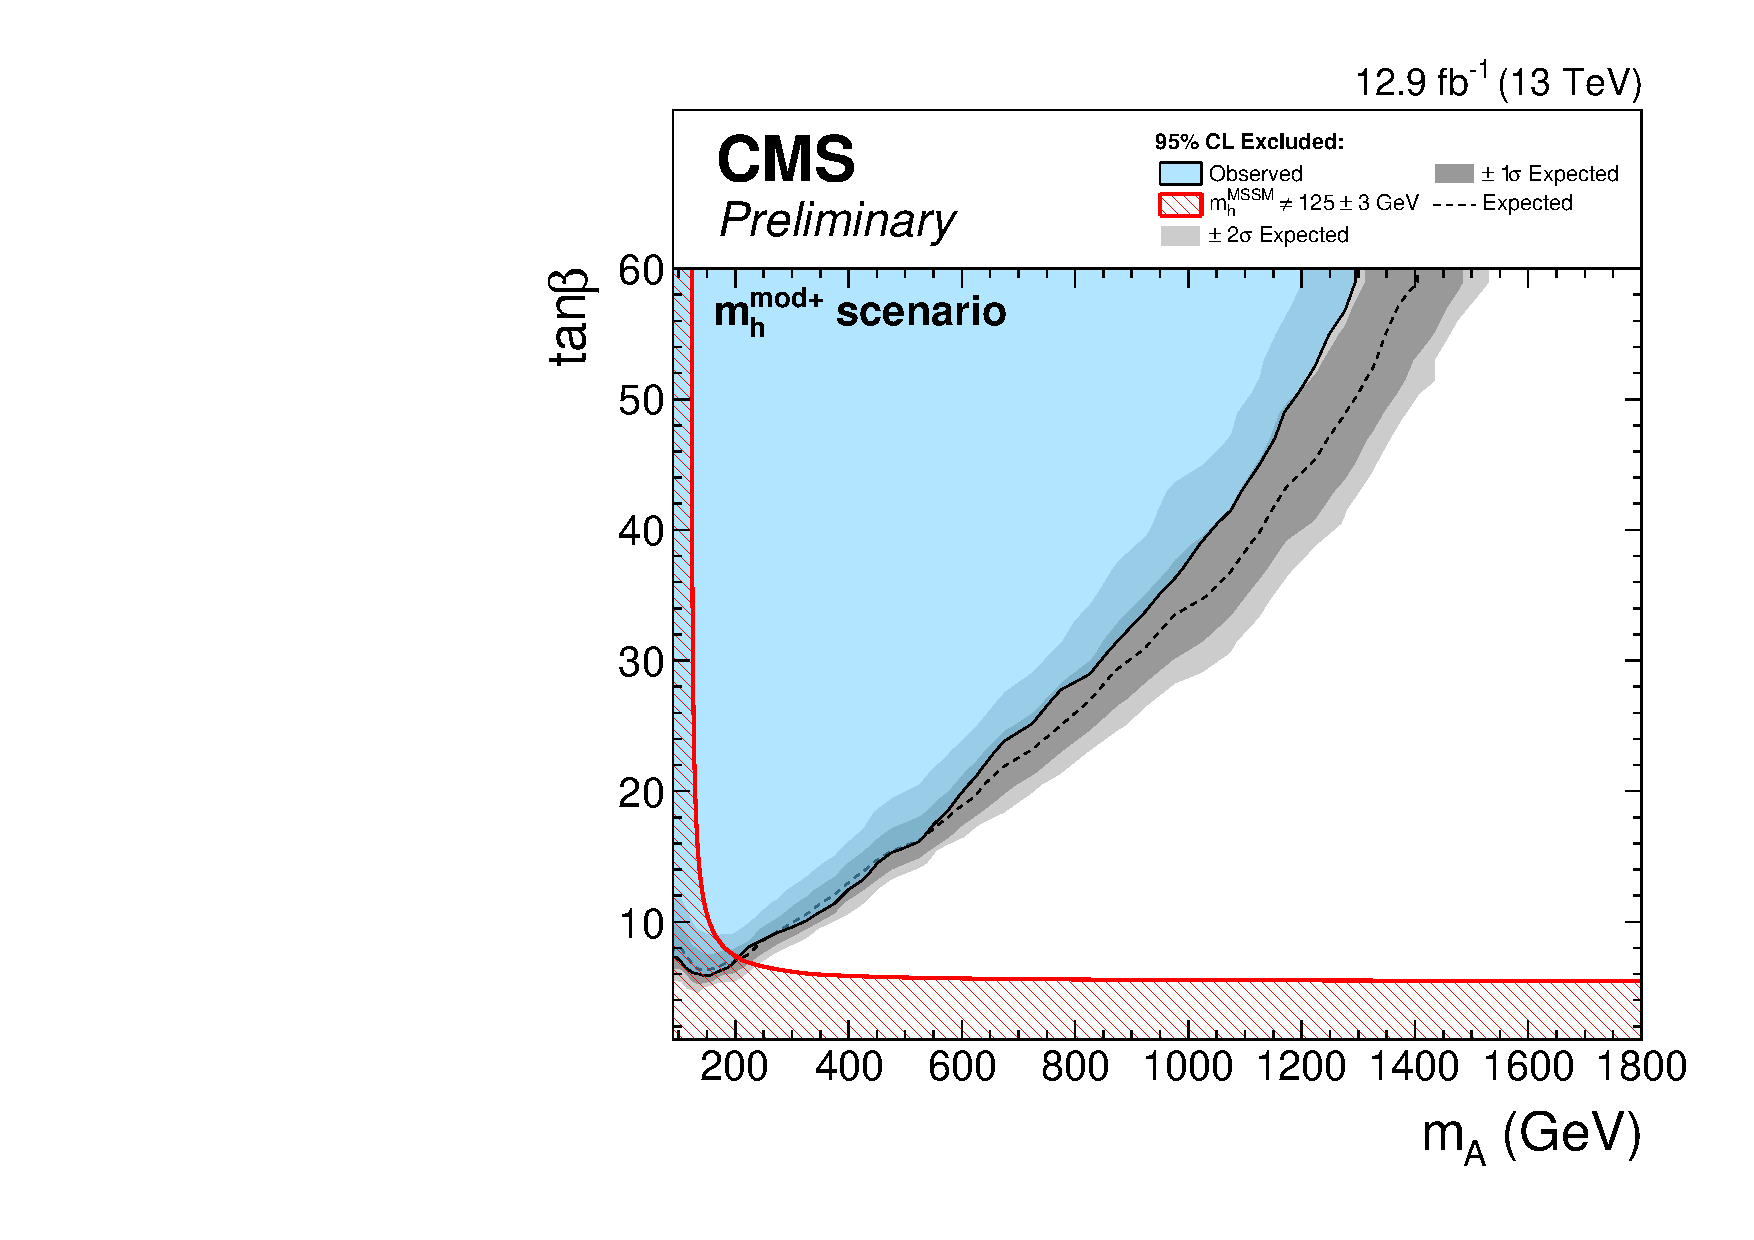
\includegraphics[width=0.7\textwidth]{./MSSM/Figures/CMS-PAS-HIG-16-037_Figure_012-a.pdf}
\end{center}
\caption{Exclusion in the $m_{h}^{\text{mod}+}$ scenario obtained by the combination
of all channels in the \AHtotautau analysis. The blue shaded area bounded by the 
solid black line is the observed exclusion, with the dashed black line the
expected exclusion. The grey bands indicate the $\pm 1,2$ $\sigma$ 
expected exclusion. The red shaded area
is excluded by the lack of a light Higgs boson with mass compatible with 125 GeV \cite{CMS-PAS-HIG-16-037}.}
\label{fig:mssm_mhmodp_2016}
\end{figure}

\begin{figure}[h!]
\begin{center}
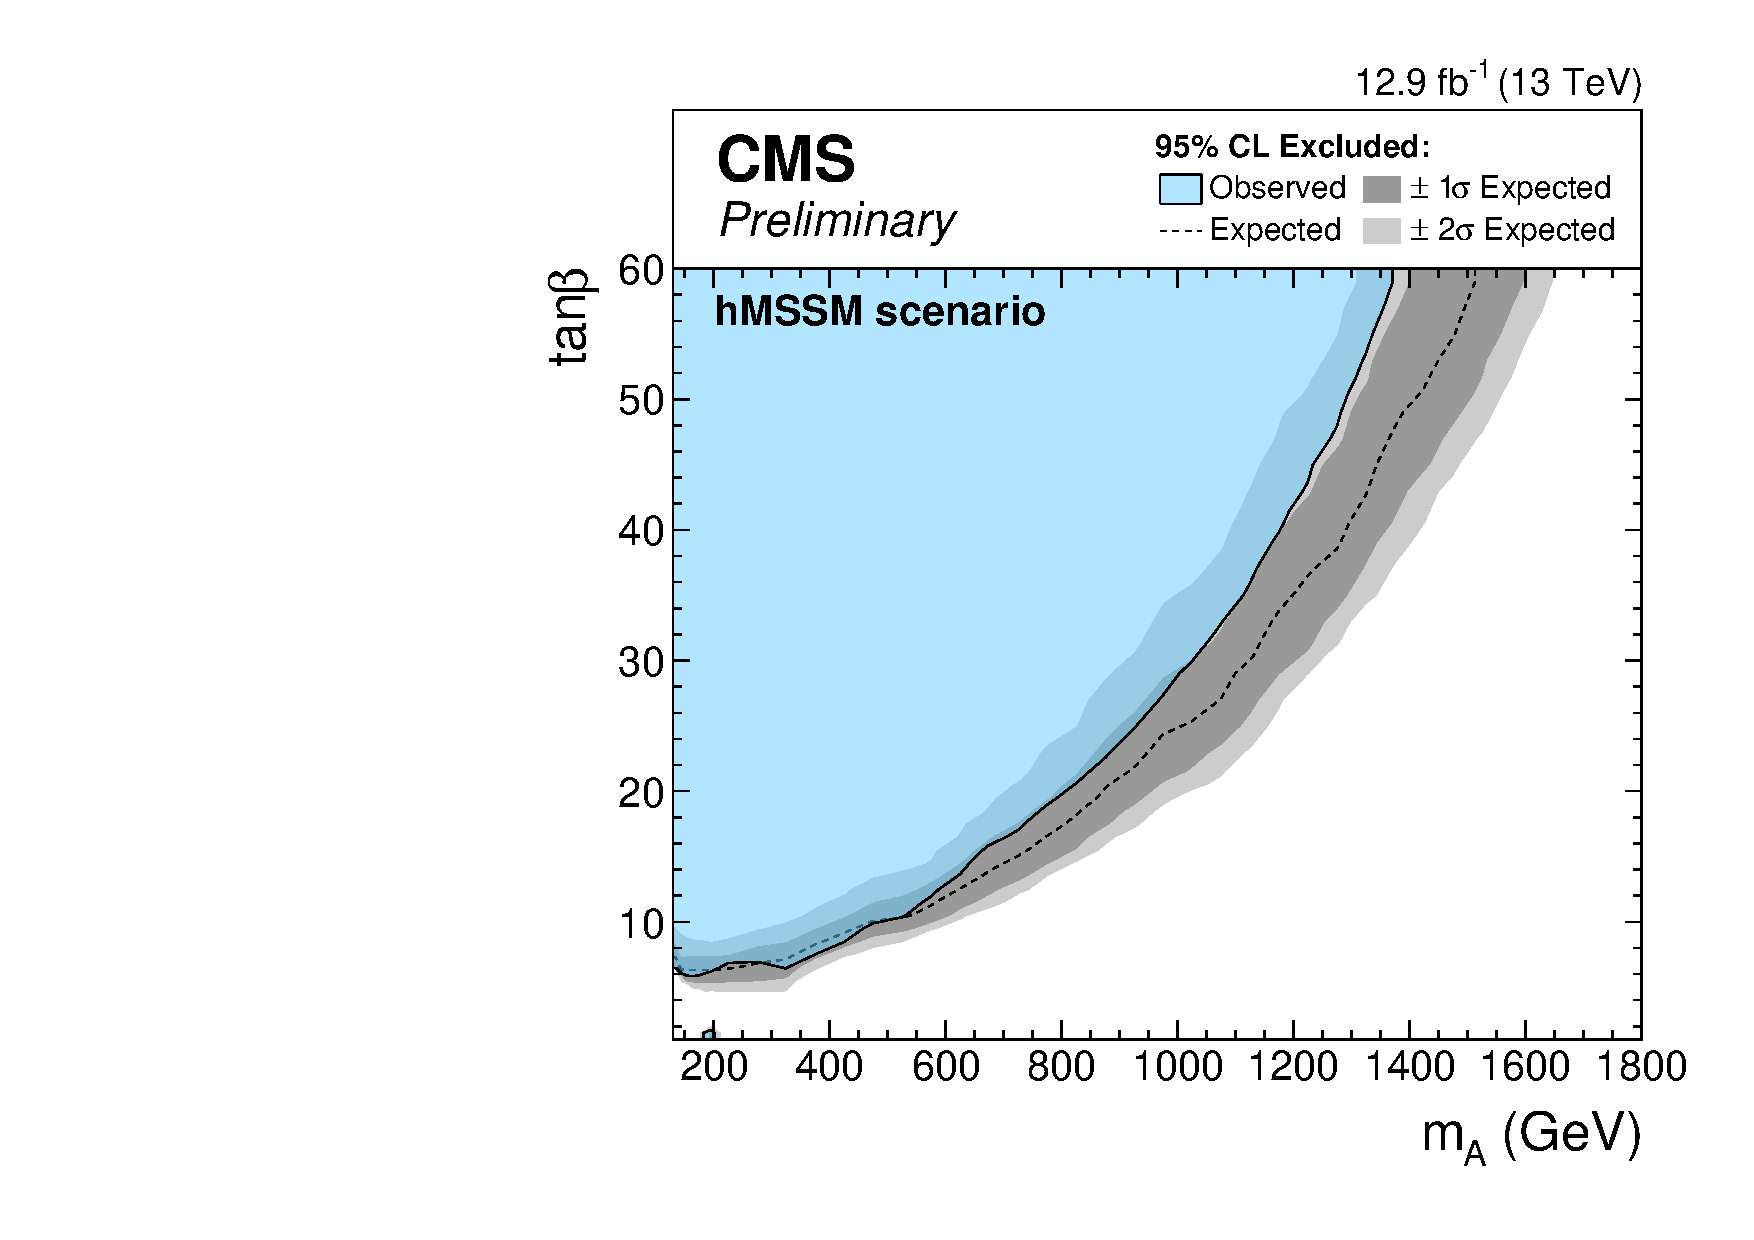
\includegraphics[width=0.7\textwidth]{./MSSM/Figures/CMS-PAS-HIG-16-037_Figure_012-b.pdf}
\end{center}
\caption{Exclusion in the hMSSM scenario obtained by the combination
of all channels in the \AHtotautau analysis. The blue shaded area bounded by the 
solid black line is the observed exclusion, with the dashed black line the
expected exclusion. The grey bands indicate the $\pm 1,2$ $\sigma$ 
expected exclusion \cite{CMS-PAS-HIG-16-037}.}
\label{fig:mssm_hmssm_2016}
\end{figure}


\section{Combination of 2015 and 2016 datasets}
\label{sec:mssm_combination}

\subsection{Procedure}
\label{sec:mssm_combination_procedure}

\subsection{Results}
\label{sec:mssm_combination_results}


